\documentclass[11pt]{article}
\usepackage[T1]{fontenc}
\usepackage[utf8]{inputenc}
\usepackage{lmodern,microtype}
\usepackage[a4paper,margin=28mm]{geometry}
\usepackage{amsmath,amssymb,amsthm,mathtools}
\usepackage{booktabs,array,enumitem,tikz,float}
\usetikzlibrary{arrows.meta,positioning}
\usepackage[numbers,sort&compress]{natbib}
\usepackage{xurl}
\usepackage[hidelinks,hypertexnames=false]{hyperref}
\hypersetup{pdftitle={A density-uniform condensate bound for dilute Bose gases},
 pdfauthor={OpenAI}}
\newtheorem{theorem}{Theorem}[section]
\newtheorem{proposition}[theorem]{Proposition}
\newtheorem{lemma}[theorem]{Lemma}
\newtheorem{corollary}[theorem]{Corollary}
\theoremstyle{definition}
\newtheorem{definition}[theorem]{Definition}
\theoremstyle{remark}
\newtheorem{remark}[theorem]{Remark}
\newcommand{\R}{\mathbb R}
\newcommand{\Z}{\mathbb Z}
\newcommand{\N}{\mathbb N}
\newcommand{\dd}{\,\mathrm d}
\DeclareMathOperator{\Tr}{Tr}
\DeclareMathOperator{\supp}{supp}
\DeclareMathOperator{\dist}{dist}
\allowdisplaybreaks[2]
\setlength{\emergencystretch}{2em}
\pdfinfoomitdate=1
\pdftrailerid{}
\pdfsuppressptexinfo=15
\title{A density-uniform condensate bound for dilute Bose gases}
\author{OpenAI}
\date{September 27, 2026}
\begin{document}
\maketitle
\begin{abstract}
For each fixed bounded measurable, nonnegative, radial interaction of finite
range in three dimensions that is not zero almost everywhere, we prove
a positive lower bound on the constant-orbital
condensate fraction that is uniform over all sufficiently small densities
and all temperatures between zero and the square of the density.
The interaction and density remain fixed in the thermodynamic limit.
\end{abstract}
\tableofcontents
\section{The model and the uniform bound}\label{sec:introduction}

For a homogeneous gas, Bose--Einstein condensation means that one orbital
contains a positive fraction of all particles in the equilibrium state.
We consider the spatially constant orbital and keep both the physical
interaction and a positive density fixed as the volume grows.
The bound below uses the same positive fraction throughout a sufficiently
dilute interval of densities.

Let $v:\R^3\to[0,\infty)$ be bounded, measurable, radial, and supported
in a ball of finite radius, with $v$ not zero almost everywhere.
On the torus $\Lambda_L=(\R/L\Z)^3$, of volume $V=L^3$, let
$v_L(x)=\sum_{k\in\Z^3}v(x+Lk)$ and define
\[
 H_{N,L}=-\sum_{i=1}^N\Delta_i+
                \sum_{1\le i<j\le N}v_L(x_i-x_j)
 \quad\hbox{on }L^2_{\mathrm{sym}}(\Lambda_L^N).
\]
The units are $\hbar^2/(2m_{\mathrm{particle}})=k_B=1$.
At $T>0$, the state is the canonical Gibbs state
$\Gamma_{N,L,T}=e^{-H_{N,L}/T}/\Tr e^{-H_{N,L}/T}$; at $T=0$, it is
the ground state. Write $\gamma^{(1)}_{N,L,T}$ for its one-particle
density matrix, normalized to trace $N$, and put $u_0=V^{-1/2}$.

\begin{theorem}\label{thm:main}
For every potential $v$ as above there are constants
$\rho_*(v)>0$ and $c_*(v)>0$ with the following property.
For every $0<\rho<\rho_*(v)$ there is $L_0(\rho,v)<\infty$ such that,
for every $L\ge L_0(\rho,v)$, every integer $N\ge1$ satisfying
$\rho/2\le N/L^3\le2\rho$, and every $0\le T\le\rho^2$,
\[
 \frac{\langle u_0,\gamma^{(1)}_{N,L,T}u_0\rangle}{N}
 \ge c_*(v).
\]
Consequently, for each such fixed density $\rho$ and fixed
$0\le T\le\rho^2$, every sequence with $L\to\infty$ and
$N/L^3\to\rho$ has lower limiting condensate fraction at least $c_*(v)$.
\end{theorem}

The volume threshold may depend on the density; the condensate lower
bound does not. The Hamiltonian is the exact interacting Hamiltonian,
and its potential is not rescaled with the number of particles.
The conclusion is macroscopic occupation of the constant orbital with
a positive lower bound throughout the admitted dilute interval. The
zero-temperature state is unambiguous: positivity of the finite-volume
heat kernel gives a unique bosonic ground state, as shown at the end
of the proof.

\subsection{Context and antecedents}
The ideal-gas theory begins with Bose's counting of light quanta
\cite{Bose1924} and Einstein's extension to a monatomic ideal gas,
including the condensation prediction in his second paper
\cite{Einstein1924IdealGas,Einstein1925IdealGas}.
Bogoliubov's treatment of weakly interacting bosons introduced an
approximate quasiparticle description based on macroscopic occupation of
one mode \cite{Bogolubov1947}.

For interacting particles, Penrose and Onsager formulated condensation
through a macroscopic eigenvalue of the one-particle density matrix and
applied this viewpoint to liquid helium \cite{PenroseOnsager1956}.
Yang developed the broader framework of off-diagonal long-range order,
covering Bose condensation and fermion pairing \cite{Yang1962ODLRO}.
These criteria identify the order to be proved; establishing it for a
specified interacting Hamiltonian remains a separate mathematical problem.

Rigorous lattice antecedents include Dyson, Lieb, and Simon's
low-temperature long-range order for the spin-$\tfrac12$ nearest-neighbor
quantum XY model on the simple cubic lattice in dimensions $d\ge3$
\cite{DysonLiebSimon1978}, and Kennedy, Lieb, and Shastry's ground-state
long-range order for all spins on hypercubic lattices in dimensions $d\ge2$
\cite{KennedyLiebShastry1988XY}.
For spin-$\tfrac12$, the spin--hard-core-boson correspondence relates
these results to condensation of half-filled lattice bosons.
Passing to a continuum Hamiltonian with a fixed interaction
and a prescribed density requires additional arguments.

The distinction between the thermodynamic and Gross--Pitaevskii limits is
essential. Lieb and Seiringer proved complete condensation in the
Gross--Pitaevskii limit, with the interaction scaled so that $Na$ remains
fixed, where $a$ is the scattering length
\cite{LiebSeiringer2002BEC}. Deuchert and Seiringer subsequently treated
positive-temperature homogeneous gases with scattering length
$a_N=a_vL/N$, where $a_v$ is the scattering length of the
unscaled potential, and controlled the one-particle density matrix of approximate
Gibbs minimizers \cite{DeuchertSeiringer2020GP}. These results allow the
interaction scale to vary with particle number. The problem considered
here instead fixes the potential and a positive density before taking
the volume to infinity.

The limits between Gross--Pitaevskii scaling and a fixed-density
thermodynamic limit have several forms. Brennecke, Brooks, Caraci, and
Oldenburg proved complete ground-state condensation in the
Gross--Pitaevskii regime and beyond
\cite{BrenneckeBrooksCaraciOldenburg2025}. Fournais treated low-energy
states on growing boxes in a joint dilute and increasing-volume limit
\cite[Theorem~1.2]{Fournais2021}. Chong, Liang, and Nam gave simpler
proofs of low-energy condensation using kinetic localization and
Poincar\'e-type inequalities \cite{ChongLiangNam2026}.
For the unit-box interaction $N^{2-2\kappa}v(N^{1-\kappa}x)$,
rescaling to a fixed potential gives density $N^{3\kappa-2}$;
the regimes $\kappa<2/3$ therefore couple dilution to increasing
particle number. Junge's low-temperature canonical Gibbs-state
result uses Neumann boxes whose size remains coupled to
the dilute limit \cite[Corollary~6]{Junge2026Propagation}.

The thermodynamic energy problem has a separate history. Dyson's
hard-sphere bounds and the leading dilute asymptotics of Lieb and
Yngvason established the first-order energy scale
\cite{Dyson1957,LiebYngvason1998}. The next correction was predicted
by Lee, Huang, and Yang's pseudopotential calculation
\cite{LeeHuangYang1957}. Fournais and Solovej proved the corresponding
lower bound for nonnegative radial finite-range potentials, including hard cores
\cite[Theorems~1.1 and~1.3]{FournaisSolovej2023}; recent upper bounds
attain the same coefficient for hard spheres and for general
nonnegative even finite-range potentials
\cite{BastiEtAl2026HardSpheres,BastiEtAl2026GeneralPotentials}.
These energy results, and low-temperature free-energy estimates for
strong potentials \cite{FournaisEtAl2026StrongFreeEnergy}, do not by
themselves determine occupation of a single orbital: the one-particle
kinetic gap tends to zero as the volume grows.

A distinct thermodynamic-limit result appears in S\"ut\H{o}'s two-step preprint
\cite{Suto2023TwoStep}. Its Theorem~1.2 assumes nonnegativity both of the
potential and of its Fourier transform, together with integrability,
a Fourier-moment condition, and spatial decay, and states condensation
above a temperature-dependent density threshold. Fourier positivity is
an additional restriction: for example, a nonnegative spherical square
barrier has a Fourier transform that changes sign. That result therefore
does not cover all bounded nonnegative radial finite-range potentials,
and its fixed-temperature threshold does not alone provide the joint
low-density and low-temperature uniformity sought here.

Galanda and Pinamonti construct algebraic equilibrium states with a
condensate background under quantitative convergence conditions for a
spatially localized interaction \cite[Theorem~6.8]{GalandaPinamonti2025Equilibrium}.
Their subsequent analysis treats renormalized correlation functions in
Gross--Pitaevskii scaling, with a zero-temperature limit in its final
convergence theorem \cite[Theorem~7.3]{GalandaPinamonti2026GP}.
These constructions use a different state formulation and coupled
interaction, regulator, and temperature limits from the fixed-potential
canonical thermodynamic limit considered here.

The trajectory formulation descends from Feynman's treatment of the
Bose gas \cite{Feynman1953AtomicLambda}; for the canonical
Feynman--Kac representation and its symmetrization and one-particle
normalizations, see \cite[Appendix~A]{Ueltschi2006FeynmanCycles}.
The random-path comparison has a different ancestry.
Benjamini, Pemantle, and Peres constructed paths with exponentially
decaying intersection tails \cite{BenjaminiPemantlePeres1998}.
H\"aggstr\"om and Mossel developed a hierarchical random-drift
construction with low predictability; its independent block variables
are a close antecedent of the dyadic velocities used below
\cite[Section~3, Proposition~3.1]{HaggstromMossel1998}.
Abbe, Massouli\'e, Montanari, Sly, and Srivastava used finite-endpoint
path averages and overlap estimates for group synchronization
\cite{AbbeMassoulieMontanariSlySrivastava2018}; Garban and Spencer used
this approach for classical disordered-spin symmetry breaking along the Nishimori line
\cite{GarbanSpencer2023}. Here the finite cell paths, their thickened
intersection estimates, and the continuum bridge comparison require
separate proofs.


\subsection{How the comparison works}

Let $q_0=\langle u_0,\gamma^{(1)}u_0\rangle/N$.
The Feynman--Kac formula expresses the partition function by positive
weights on closed collections of paths. Replacing one matching endpoint
by an independently integrated spatial point gives a positive measure
$\mu$ of total mass $q_0$. We construct a measure $\nu$ by changing a
short portion of closed paths, with mass at least a fixed $a>0$, and
show that its density $f=\dd\nu/\dd\mu$ has bounded second moment.
Cauchy--Schwarz then gives
\[
                    a^2\le q_0\int f^2\dd\mu.
\]
Thus the main problem is a comparison of positive path measures.

Partition space into cells of side $s$ comparable to $\rho^{-1/2}$,
and change paths only during a time interval of length $\delta=s^2$.
The mean count $m=Ns^3/V$ is comparable to $\rho^{-1/2}$, making
many particle choices available in a typical cell as the density decreases,
while the slab remains short compared with $1/T$ throughout the
positive-temperature range.

The local analysis must control simultaneous failures in specified
families of cells. Energy and entropy estimates first give occupation
tails and separation of most endpoints at the shorter scale
$r=\zeta\rho^{-1/3}$, with $\zeta>0$ fixed and small. A particle is
eligible when its endpoints are separated, its path stays near them
during short initial and final time intervals, and it satisfies overall
confinement and integrated interaction-score bounds for the path
ensemble. The interacting
bridges are not independent. A separate localized partition-function
comparison bounds their joint trajectory failures, with a cost
proportional to the volume of the tested cells. Together with the
one-time estimates and score bounds, this makes specified sets of
unusable cells unlikely.

Between two distant cells, choose a random lattice path, called a
skeleton, whose encounters with an independent copy have bounded
exponential moments. Here an encounter records a vertex within a
fixed cell distance of the other path; a second estimate weights all
vertices by exponentially decaying distance. These two geometric
bounds are established independently of the gas in
Section~\ref{sec:skeletons}. Detour around unusable components. Select one eligible particle from
each cell on the resulting simple path, and cyclically reassign their
starting points. One end is opened and the selected bridges are sampled
from their exactly normalized interacting law. This defines $\nu$.

The second moment involves two independently chosen paths in related
configurations. Estimating both changes against the original closed
configuration would incur a cost proportional to their lengths.
Instead, a reverse insertion supplies a baseline in which contributions
far from encounters cancel. Two effects remain small as $\rho$ decreases:
an encounter of distinct separated bridges has interaction cost tending
to zero at rate $r^{-1/2}$, and coincident particle choices have probability
of order $1/m$.

Changing trajectories also changes which cells are usable and which
particles are eligible, so the two routes cannot be treated as independent
of the gas. A stricter cell test in the reverse configuration controls
these changes: away from encounters the selection weights agree, while
rare components give a controlled list of possible detours. Keeping
those selection weights throughout the comparison yields the required
second-moment bound after averaging over the environment and the two
paths.

Sections~\ref{sec:energy}--\ref{sec:defects} prove the local analytic
bounds. Section~\ref{sec:geometry} constructs the paths and detours.
Section~\ref{sec:opening} defines the change of measure, and
Section~\ref{sec:comparison} proves its second-moment estimate with all
normalizations and selection constraints retained.
Section~\ref{sec:conclusion} fixes the parameters in order and passes
the uniform positive-temperature bound to zero temperature.

\section{Scales and conventions}\label{sec:setup}

We use the Hamiltonian of Section~\ref{sec:introduction} also on labelled
coordinates, and suppress $L$ when it is fixed. We choose an everywhere
nonnegative bounded Borel radial representative of $v$ vanishing outside
its range ball. Changing this representative on a null set changes neither
the operator nor the path integrals: at interior times the free relative
positions have densities. Write $R_v$ for a range bound, and use
$\|v\|_1,\|v\|_\infty$ on $\R^3$. In formulas on the torus,
$v$ abbreviates its periodization $v_L$; infinite-space norms always
refer to the original potential.

The orthogonal symmetrizer is included exactly once in a trace kernel.
If $k_t$ is the labelled $N$-particle kernel, then
\[
 k_t^{\mathrm{sym}}(X,Y)=\frac1{N!}\sum_{\pi\in\mathfrak S_N}
                         k_t(X,\pi Y),\qquad
 Z_N=\int k_\beta^{\mathrm{sym}}(X,X)\dd X.
\]
Thus integration over labelled coordinates carries no further factorial.
We work with $\rho/2\le N/V\le2\rho$, $0<T\le\rho^2$, and
$\beta=T^{-1}$. Every volume restriction below is imposed at fixed $\rho$,
uniformly over this temperature interval. Constants $C,c>0$ may change
between occurrences and depend on $v$ and previously fixed cutoffs,
but not on $\rho,L,N,T$. The final order of those cutoff choices is
recorded in Section~\ref{sec:conclusion}.

We use a periodic grid \(\mathcal G=(\mathbb Z/n\mathbb Z)^3\) of equal cubes (fix the assignment at faces), with
\[
 n=\left\lfloor\frac{L}{K\rho^{-1/2}}\right\rfloor,\qquad
 s=L/n\in[K\rho^{-1/2},2K\rho^{-1/2}],\qquad
 M=n^3,\quad m=N/M .
\]
Here \(K\ge1\) is a fixed large constant chosen below. Thus \(\rho s^3/2\le m\le 2\rho s^3\). 

A union \(U\) of \(u\ge1\) cells has volume \(|U|=u s^3\). A neighborhood out to distance \(h s\), \(h\ge0\), can be covered by at most \(C(h+2)^3 u\) cells, including on the torus. Physical distances \(d(\cdot,\cdot)\) are Euclidean torus distances unless indicated otherwise. Cell index distances will use the periodic sup norm. For a function \(p\) of position put \(n_p(X)=\sum_i p(x_i)\) on configurations (also the multiplication operator); similarly \(n_U\) for counting particles in \(U\).


\section{Energy and free-energy estimates}\label{sec:local-energy}\label{sec:energy}

This section gives the particle-number costs needed to localize the gas.
Throughout, $0<T\leq\rho^2$, $\beta=T^{-1}$, and
$\rho/2\leq N/V\leq2\rho$. All statements hold after decreasing a
potential-dependent upper bound on $\rho$ and increasing the volume
threshold at each fixed density. The Hamiltonian with a bounded external
potential $-W$ is denoted by $H_{j,L}^{(-W)}$; its symmetric partition
function and free energy are $Z_j^{(-W)}$ and
$F_j^{(-W)}=-T\log Z_j^{(-W)}$. We set $Z_0=1$ and $F_0=0$.
For a trace-one state $\sigma$, write
$\mathcal F^{(-W)}(\sigma)=\operatorname{Tr}H^{(-W)}\sigma-TS(\sigma)$.
Here $S(\sigma)=-\operatorname{Tr}(\sigma\log\sigma)$ is the
von Neumann entropy, with $0\log0=0$.
Constants may depend on $v$, and later on already fixed dimensionless
parameters, but never on $\rho,L,N,T$.

\begin{lemma}[A Neumann cell bound]\label{lem:neumann-cell}
There are $b_0,c_v>0$, depending only on the fixed potential, such that
for a cube $Q$ of side $b\geq b_0$, every $y\in Q$, and every
$f\in H^1(Q)$,
\begin{equation}
 \int_Q\bigl(|\nabla f|^2+v(x-y)|f|^2\bigr)\,dx
 \geq c_v b^{-3}\int_Q|f|^2\,dx.\tag{1}\label{eq:1}
\end{equation}
The same conclusion holds for fixed positive coefficients in front of
the two terms, with changed constants. Consequently, for disjoint
cubes $Q$ of common side $b$, kinetic energy plus nonnegative pair
energy bounds below the multiplication operator
\begin{equation}
 c_v b^{-3}\sum_Q n_Q\mathbf1_{\{n_Q\geq2\}}.\tag{2}\label{eq:2}
\end{equation}
Both statements apply to torus cubes smaller than the torus, and to
Dirichlet states extended by zero.
\end{lemma}

\begin{proof}
Choose $\nu>0$ for which the radial set
$A=\{x:v(x)\geq\nu\}$ has positive measure. Increase $b_0$ so that
$b_0/2>R_v$ and $b_0\geq1$. For each $y\in Q$ choose, independently
in the three coordinate directions, an orientation with available
length at least $b/2$. The resulting octant of $y+A$ lies in $Q$ and
has measure $|A|/8=:a_v>0$ by radial symmetry. Call it $A_y$.
For $f_0=|Q|^{-1}\int_Q f$, the scale-invariant Sobolev--Poincar\'e
inequality gives $\|f-f_0\|_6\leq C\|\nabla f\|_2$. Thus
\[
 a_v|f_0|^2\leq2\int_{A_y}|f|^2+
 2\int_{A_y}|f-f_0|^2
 \leq2\nu^{-1}\int_Qv(x-y)|f|^2+
 C a_v^{2/3}\int_Q|\nabla f|^2.
\]
Moreover $\|f-f_0\|_2^2\leq Cb^2\|\nabla f\|_2^2$.
Since $b^2\leq b^3$ for $b\geq1$, these estimates give (1).
Positive fixed energy coefficients only change the constants.

For (2), cut configuration space according to the cube containing
each coordinate and discard cross-cube interactions. This is Neumann
bracketing: the restrictions of an $H^1$ function to the pieces are
admissible with no boundary condition at the cuts. Within a cube
containing $j\geq2$ coordinates, pair them disjointly. For each pair
apply (1) in the first coordinate with the other coordinate held
fixed, and then integrate the other coordinates. No coordinate
kinetic term or pair interaction is used twice. The number of pairs
is $\lfloor j/2\rfloor\geq j/3$. Summing the resulting inequalities
proves (2). The argument is unaffected by additional nonnegative
periodic images of $v$. Zero extension gives the Dirichlet assertion.
\end{proof}

\begin{lemma}[An entropy bound]\label{lem:kinetic-entropy}
If $\Omega$ is an open subset of the torus with Dirichlet kinetic
energy, or the full torus with periodic kinetic energy, then for
every $\alpha>0$ and every finite-energy symmetric trace-one $j$-particle state,
\begin{equation}
 \alpha\operatorname{Tr}\Bigl(\sum_{i=1}^j-\Delta_i\Bigr)\sigma
 -TS(\sigma)
 \geq-Tj-C_\alpha T|\Omega|(V^{-1}+T^{3/2}).\tag{3}\label{eq:3}
\end{equation}
In particular a state of finite kinetic energy has finite entropy.
\end{lemma}

\begin{proof}
The periodic heat kernel satisfies
$K_t(0)\leq C(V^{-1}+t^{-3/2})$ by its Gaussian image sum,
or equivalently by its Fourier series. Killing at $\partial\Omega$
decreases its diagonal, so
$\operatorname{Tr}e^{t\alpha\Delta_\Omega}
\leq C_\alpha|\Omega|(V^{-1}+t^{-3/2})$.
The ideal Bose grand partition function with fugacity $e^{-1}$ has
logarithm
\[
 \sum_{l\geq1}\frac{e^{-l}}l
 \operatorname{Tr}e^{l\beta\alpha\Delta_\Omega}
 \leq C_\alpha|\Omega|(V^{-1}+T^{3/2}).
\]
Its $j$-particle term is $e^{-j}$ times the canonical partition
function. Applying the Gibbs variational inequality to that term
gives (3). For an arbitrary finite-energy state, the same inequality
follows first on finite spectral truncations and then by monotone
entropy approximation, or directly from nonnegativity of relative
entropy to the ideal Gibbs state. The right side is finite, proving
the entropy assertion as well.
\end{proof}

\begin{proposition}[Particle-number free-energy bounds]\label{prop:increments}
Uniformly in the temperature range under consideration,
\begin{align}
 F_N&\geq c_v\rho N,\tag{4}\label{eq:4}\\
 F_{N+k}&\geq F_N+c_v\rho k\qquad(k\geq0).\tag{5}\label{eq:5}
\end{align}
For every bounded $W\geq0$, with no upper bound on its size required,
\begin{equation}
 F_j^{(-W)}-F_{j-1}^{(-W)}\leq C_v\rho
 \qquad(1\leq j\leq4\rho V).\tag{6}\label{eq:6}
\end{equation}
The constant in (6) is independent of $W$.
\end{proposition}

\begin{proof}
Partition the torus into equal cubes of side in $[b,2b]$, where
$b=(4/\rho)^{1/3}$. The number of cubes is at most
$V/b^3=\rho V/4\leq N/2$ when $L$ is sufficiently large.
Reserve a fixed fraction of kinetic energy for (3), and apply (2)
to the rest of the kinetic energy and the interaction. Since
$\sum_Q n_Q\mathbf1_{\{n_Q\geq2\}}\geq N-\#\{Q\}\geq N/2$,
the energy contribution is at least $c_v\rho N$.
The entropy loss is bounded by
$TN+C T(1+VT^{3/2})$. Divided by $\rho N$, these terms tend uniformly
to zero as $\rho\downarrow0$ and the volume threshold increases:
$T/\rho\leq\rho$, $T/(\rho N)\leq\rho/N$, and
$VT^{5/2}/(\rho N)\leq2\rho^3$. This proves (4), after changing $c_v$.

We next show that $F_j/j$ is nondecreasing in $j\geq1$.
Regard a symmetric $j$-particle state as a state on the labeled tensor
product and denote by $S_i$ the entropy of its trace-one
$i$-particle marginal; put $S_0=0$. Strong subadditivity~\cite[Theorem~2 and Section~IV]{LiebRuskai1973Entropy} applied to
two overlapping $i$-coordinate subsystems with overlap of size
$i-1$ gives $2S_i\geq S_{i-1}+S_{i+1}$. The case $i=1$ uses
ordinary subadditivity. Permutation symmetry identifies the
marginals occurring here. Therefore $S_i$ is concave and
$S_j/j\leq S_{j-1}/(j-1)$ for $j\geq2$.
The one-body energy per particle is unchanged by passage to the
$(j-1)$-particle marginal. The pair energy per particle decreases,
because its coefficient is $(j-1)/2$ before passage and $(j-2)/2$
afterwards, and the common two-body expectation is nonnegative;
for $j=2$ the latter energy is zero. The marginal remains supported
on the symmetric subspace. Applying these observations to the Gibbs
state and then using its marginal as a variational state proves
$F_j/j\geq F_{j-1}/(j-1)$. All entropies are finite by (3).
Consequently
$F_{N+k}\geq(N+k)F_N/N$, which with (4) proves (5).

The lower increments now quantify the free-energy gain from adding
particles. To obtain the complementary upper cost, uniformly even in
an attractive external field, we insert one particle directly in the
path representation.

Retain in the symmetrized Feynman--Kac
formula only those permutations in which the extra label is fixed.
There are $(j-1)!$ such permutations against the factor $1/j!$.
The added particle is a free torus loop whose start is integrated
over the torus. After normalization by $VK_\beta(0)$ its position
at every time is uniform, independently of all old trajectories.
Thus its expected total interaction with the old paths is
$\beta(j-1)\|v\|_1/V$. Its external weight is at least one because
$W\geq0$. Jensen's inequality, conditional on all old paths, gives
\[
 Z_j^{(-W)}\geq\frac{VK_\beta(0)}j
 e^{-\beta(j-1)\|v\|_1/V}Z_{j-1}^{(-W)}.
\]
Since $K_\beta(0)\geq(4\pi\beta)^{-3/2}$, the positive part of the
prefactor's contribution to the increment is bounded by
$T\log_+(C\rho T^{-3/2})$. For small $\rho$, the derivative of
$t\mapsto t\log(C\rho t^{-3/2})$ on $0<t\leq\rho^2$ is
$\log(C\rho t^{-3/2})-3/2\geq\log(C\rho^{-2})-3/2>0$.
Its maximum on this interval is therefore at most
$C\rho^2(1+|\log\rho|)\leq C\rho$.
The interaction contribution is at most $4\|v\|_1\rho$.
This proves (6), uniformly even as $T\downarrow0$.
\end{proof}

\section{Localization, occupation, and isolation}\label{sec:localization}

We now obtain simultaneous probability bounds for specified collections
of cells. The important scale is $s\asymp K\rho^{-1/2}$: a cell contains
$m=Ns^3/V\asymp\rho s^3$ particles on average, and $m$ tends to infinity
as the density decreases. All cutoffs below are real and Lipschitz;
their gradients and the resulting form identities are understood
almost everywhere.

The estimates use the same variational comparison. Spatial localization
gives a lower bound for the free-energy cost of a tilted state, while
diagonal tilting gives an upper bound for that cost in terms of a gradient
error and the tilt's normalization. Comparing the two bounds controls
the derivative of a logarithmic exponential moment. Positive density
tilts control excess occupation, negative tilts control shortages, and
a tilt of the close-particle count will give isolation.

\begin{lemma}[Two-color localization and diagonal tilting]\label{lem:localization-tilt}
Let $p^2+q^2=1$, and suppose multiplication by $p$ maps the one-particle
form domain into $H^1_0(\Omega)$ for an open region $\Omega$.
For a finite-energy symmetric trace-one $J$-particle state $\sigma$, let $w_j$ be
the distribution of the number of particles in the $p$ color, and
let $\sigma_{\mathrm{in},j},\sigma_{\mathrm{out},j}$ be the two
conditional marginal states. Then
\begin{equation}
 \mathcal F^{(-W)}(\sigma)+\operatorname{Tr}
 n_{|\nabla p|^2+|\nabla q|^2}\sigma
 \geq\sum_{j=0}^Jw_j\bigl[
 \mathcal F^{(-W)}(\sigma_{\mathrm{in},j})+
 \mathcal F^{(-W)}(\sigma_{\mathrm{out},j})\bigr]-TH(w).
 \tag{7}\label{eq:7}
\end{equation}
Here $H(w)=-\sum_jw_j\log w_j$, with $0\log0=0$, is the Shannon
entropy, and $H(w)\leq C+\sum_jjw_j$ and
$\sum_jjw_j=\operatorname{Tr}n_{p^2}\sigma$.

Let $\Gamma=Z_N^{-1}e^{-\beta H_{N,L}}$, let $P$ be its position
law, and let $G$ be a bounded symmetric Lipschitz real function of
positions. Put $g=e^G$, $M_G=\mathbb E_Pe^{2G}$ and
$\sigma=g\Gamma g/M_G$. For expectation under its position law
write $\mathbb E_g$. Then
\begin{equation}
 \mathcal F(\sigma)-F_N\leq
 \mathbb E_g\sum_i|\nabla_iG|^2+
 T\bigl(2\mathbb E_gG-\log M_G\bigr).
 \tag{8}\label{eq:8}
\end{equation}
\end{lemma}

\begin{proof}
The geometric localization and entropy split behind (7) also appear in
\cite[Section~3, Lemma~3.1]{DeuchertSeiringerYngvason2019}.
We give the decomposition into fixed color-number sectors explicitly.
The one-particle map $f\mapsto(pf,qf)$ is an isometry into the direct
sum of the two one-particle spaces. Its symmetric tensor power is
therefore an isometry. Dephase the resulting state with respect to
the first-color number. The $j$-sector is unitarily identified with
$\operatorname{Sym}^jL^2(\Omega)\otimes
\operatorname{Sym}^{J-j}L^2(\Lambda_L)$: normalized symmetrization
over color assignments gives this unitary, because the assignments
are orthogonal. In particular there is no additional multiplicity
or binomial entropy term. The product rule and
$p\nabla p+q\nabla q=0$ give exactly the kinetic error in (7).
Retain the same-color pair interactions and drop the other ones;
nonnegativity makes this an energy decrease. One-body potentials
are preserved in sum. Isometry preserves entropy, dephasing cannot
decrease it, and subadditivity in each sector bounds it by
$H(w)+\sum_jw_j[S(\sigma_{\mathrm{in},j})+
S(\sigma_{\mathrm{out},j})]$. This proves (7).
Comparison of $w$ with the geometric law
$(1-e^{-1})e^{-j}$ gives $H(w)\leq-\log(1-e^{-1})+\mathbb E j$.
Conditional on a labeled position configuration, the color choices
are independent, with probabilities $p(x_i)^2$ and $q(x_i)^2$.
This proves the number formula and also the diagonal interpretation
of every color count used below. Finite-energy approximation and
Lemma~\ref{lem:kinetic-entropy} justify all the entropy operations.

For (8), define
$\tau=\Gamma^{1/2}g^2\Gamma^{1/2}/M_G$.
The nonzero spectra of $\tau$ and $\sigma$ agree: they are the
spectra of $B^*B$ and $BB^*$ for $B=g\Gamma^{1/2}/\sqrt{M_G}$.
If $H\psi=E\psi$, testing the eigenvalue equation with $g^2\psi$
gives the form identity
\[
 \langle g\psi,Hg\psi\rangle
 =E\langle\psi,g^2\psi\rangle+
 \langle\psi,\sum_i|\nabla_i g|^2\psi\rangle.
\]
After summing in an eigenbasis,
$\operatorname{Tr}H\sigma=\operatorname{Tr}H\tau+
\mathbb E_g\sum_i|\nabla_iG|^2$. Both energies and entropies are
finite, since $g$ and its gradients are bounded at fixed $N,L$.

To compare relative entropies, approximate $g^2$ uniformly by positive
simple functions on finite partitions into symmetric measurable
sets $E$. Set $p_E=\operatorname{Tr}\Gamma\mathbf1_E$ and, for
$p_E>0$, $\tau_E=\Gamma^{1/2}\mathbf1_E\Gamma^{1/2}/p_E$.
The unmodified and tilted states are mixtures of the same $\tau_E$,
with weights $p_E$ and $p_Eg_E^2/M_G$. Monotonicity of relative
entropy under discarding the classical label (a partial trace;
see \cite[Corollary~(3.2) and Section~IV]{LiebRuskai1973Entropy}) therefore bounds
$D(\tau\Vert\Gamma)$ for this approximation by the classical
relative entropy of these weights. Uniform approximation gives
trace-norm convergence of the states and convergence of the
classical entropies, since $g$ is bounded above and away from zero.
Lower semicontinuity then gives
$D(\tau\Vert\Gamma)\leq2\mathbb E_gG-\log M_G$.
Finally $\mathcal F(\tau)-F_N=TD(\tau\Vert\Gamma)$ proves (8).
\end{proof}

For a nonempty union $U$ of coarse cells, set
$\phi_U(x)=e^{-d(x,U)/s}$, where distance is the Euclidean torus
distance. A neighborhood of radius $hs$ around $U$ is covered by
at most $C(h+2)^3$ times as many cells as $U$.

\begin{lemma}[Localized density bounds]\label{lem:density-tilts}
Let $D_0=H_0\rho$, where $H_0$ is a sufficiently large fixed number.
For $J\leq N$, $0\leq W\leq\rho$, and every finite-energy
symmetric trace-one $J$-particle state,
\begin{equation}
 \mathcal F^{(-W)}(\sigma)-F_J^{(-W)}
 \geq(c_vD_0-C_v\rho-Cs^{-2})\mathbb E_\sigma n_{\phi_U}
       -C_vD_0^2|U|.\tag{9}\label{eq:9}
\end{equation}
In the corresponding equilibrium state,
\begin{equation}
 \mathbb E n_U\leq C_v\rho|U|.\tag{10}\label{eq:10}
\end{equation}
For the unmodified $N$-particle position law,
\begin{equation}
 \log\mathbb E_Pe^{2\lambda n_{\phi_U}}
 \leq C_v\lambda\rho|U|\qquad(0\leq\lambda\leq1).
 \tag{11}\label{eq:11}
\end{equation}
In particular $\mathbb E_P n_Q^2\leq C m^2$ for every cell $Q$.
The proof of (9) can reserve a fixed positive fraction of the
inside kinetic and pair energy for a further nonnegative lower bound.
\end{lemma}

\begin{proof}
For $h\geq0$ take $p_h=1$ at distance at most $hs$ from $U$,
and interpolate by a cosine to zero between distances $hs$ and
$(h+1)s$. Set $q_h=(1-p_h^2)^{1/2}$ using the corresponding sine.
Both gradients vanish off this transition and
$|\nabla p_h|^2+|\nabla q_h|^2\leq Cs^{-2}$ there. Choose
an open support region $\Omega_h$ inside the $(h+2)s$
neighborhood; if that neighborhood covers the torus, use the torus.
Its volume is at most $C(h+4)^3|U|$.

Apply (7). Inside, partition the torus into cubes of side in
$[D_0^{-1/3},2D_0^{-1/3}]$. For small density this side is between
$b_0$ and $s$. The cubes meeting $\Omega_h$ number at most
$CD_0(h+4)^3|U|$. Applying (2) to part of the inside energy of
zero-extended Dirichlet states gives
$c_vD_0j-CD_0^2(h+4)^3|U|$.
Another fixed fraction of kinetic energy gives (3). An additional
fixed fraction may remain unused. The external potential costs at
most $\rho j$. Outside, (6) gives
$F_{J-j}^{(-W)}\geq F_J^{(-W)}-C_v\rho j$.
The classical entropy of the color number costs at most $T(C+j)$.
Since $T\leq\rho^2$, all coefficients of $j$ other than
$c_vD_0$ are bounded by $C_v\rho$. All volume errors, including
$CT[1+|\Omega_h|(V^{-1}+T^{3/2})]$, are at most
$C_vD_0^2(h+4)^3|U|$ after reducing the density: here
$|U|\geq s^3$ and $V\geq s^3$.

Average in $h$ with probability density $e^{-h}\,dh$. At each $x$,
$\int_0^\infty p_h(x)^2e^{-h}\,dh\geq\phi_U(x)$.
The averaged gradient cost is at most $Cs^{-2}\phi_U(x)$:
the transition can occur only for
$h\in[\max(0,d(x,U)/s-1),d(x,U)/s]$.
The moment of $(h+4)^3$ is finite. Taking $H_0$ large makes
$c_vD_0-C_v\rho$ positive and yields (9).
In equilibrium the left side is zero; because
$n_U\leq n_{\phi_U}$ this proves (10).

For (11), take $G=\lambda n_{\phi_U}$ in (8).
The distance function is one-Lipschitz, so
$\sum_i|\nabla_iG|^2\leq\lambda^2s^{-2}n_{\phi_U}$.
Also $G\geq0$, hence $\log M_G\geq0$ and the entropy term is
at most $2T\lambda\mathbb E_g n_{\phi_U}$.
Comparison with (9), increasing the fixed $H_0$ if necessary,
absorbs both terms and gives
$\mathbb E_g n_{\phi_U}\leq C_v\rho|U|$ uniformly in
$0\leq\lambda\leq1$. Integrate
$\partial_\lambda\log M_G=2\mathbb E_g n_{\phi_U}$
from zero to obtain (11).
For a single cell, exponential Markov gives
$P(n_Q\geq t)\leq\min(1,e^{Cm-2t})$.
Integration of $2tP(n_Q>t)$ gives $\mathbb E n_Q^2\leq C(m+1)^2$,
which is at most $Cm^2$ since $m\to\infty$ uniformly with dilution.
\end{proof}

The mean bound alone does not guarantee that a cell supplies a particle
to a spatial route. We next control simultaneous shortages and excesses
in any specified family of cells. The lower tail uses the free-energy
gain from placing extra particles in an underoccupied region; the upper
tail follows from the exponential density estimate.

\begin{lemma}[Simultaneous lower and upper occupation tails]\label{lem:occupation-tails}
There are fixed $0<b_-<1/4$ and $b_+>4$ such that for every union
$U$ of $u\geq1$ specified cells, each of the events
$\{n_Q<2b_-m\text{ for every }Q\subset U\}$ and
$\{n_Q>b_+m/2\text{ for every }Q\subset U\}$ has probability at most
\begin{equation}
 C e^{-cmu}.\tag{12}\label{eq:12}
\end{equation}
The constants and the required large fixed $K$ depend only on $v$.
\end{lemma}

\begin{proof}
In each cell of $U$ choose $p=1$ on the central cube of half-side
$s/4$, vanishing outside the central cube of half-side $s/3$.
Cosine--sine interpolation gives squared localization cost at most
$Cs^{-2}$ on these supports. Choose a squared smooth cutoff
$0\leq\phi\leq1$, supported in the cell interiors, equal to one
on these supports, with $|\nabla\phi|^2\leq C\phi/s^2$.
The union of cell interiors is the Dirichlet region for $p$.
Take one normalized smooth bump in each central cube of half-side
$s/8$ and sum the bumps with equal amplitude to get a normalized
orbital $\varphi$. Then
$\int|\nabla\varphi|^2\leq Cs^{-2}$ and
$\|\varphi\|_\infty^2\leq C/|U|$.
For small density, its support has distance greater than $R_v$
from $\operatorname{supp}q$.

The conditional outside state is supported in
$(\operatorname{supp}q)^{N-j}$, directly from the coloring map.
In a color sector with $j$ inside particles, add $k$ particles in
$\varphi$ to the outside state. The map on outside wave functions is
\[
 \psi\longmapsto
 \binom{N-j+k}{k}^{1/2}P_{\mathrm{sym}}
 (\psi\otimes\varphi^{\otimes k}).
\]
Distinct assignments of the new labels have disjoint supports, so
this is an isometry. It preserves entropy and has additive kinetic
energy; the separated supports also eliminate all old--new
interactions. A new--new pair has expectation at most
$\|v\|_1\|\varphi\|_\infty^2$. Therefore
\[
 \mathcal F(\sigma_{\mathrm{out},j})
 \geq F_{N-j+k}-Ck/s^2-C_vk^2/|U|.
\]
Choose a sufficiently small fixed $\eta>0$ and put
$k=\lfloor\eta\rho|U|\rfloor$.
Since $\rho|U|\geq\rho s^3\to\infty$, small density ensures
$k\geq\eta\rho|U|/2$, and $N+k\leq4\rho V$.
By (5), followed by (6) for $j$ backward steps,
$F_{N-j+k}\geq F_N+c_v\rho k-C_v\rho j$.
Use (3) and positivity inside. Choose $\eta$ small enough to absorb
$C_vk^2/|U|$ and then $K$ large enough to absorb $Ck/s^2$ into a
fixed fraction of $c_v\rho k$. The remaining entropy errors are
small compared with $\rho^2|U|$ for small density.
Applying (7) and using $p^2\leq\phi$ gives, for every state to
which the argument is applied,
\[
 \mathcal F(\sigma)-F_N
 \geq c_v'\rho^2|U|-C_v\rho\mathbb E_\sigma n_\phi.
\]
Here the localization term has been absorbed in the latter error,
since $s^{-2}\leq\rho/K^2$.

Now set $G=-\lambda n_\phi$, $0\leq\lambda\leq1$, in (8).
Its gradient contribution is at most
$C\lambda^2s^{-2}\mathbb E_gn_\phi$; its entropy contribution is
at most $-T\log M_G$, because $G\leq0$.
Thus, after changing constants,
$C_v\rho\mathbb E_g n_\phi-T\log M_G\geq c_v'\rho^2|U|$.
Put $f(\lambda)=-\log M_G$. It is nondecreasing and
$f'(\lambda)=2\mathbb E_gn_\phi$. While
$f(\lambda)\leq a\rho|U|$, one has
$Tf(\lambda)\leq a\rho^3|U|$, so for sufficiently small density
$f'(\lambda)\geq c_v''\rho|U|$. Choose fixed
$0<a<c_v''$. Starting at $f(0)=0$, this differential inequality
forces $f(1)\geq a\rho|U|$. We have proved
$\mathbb E e^{-2n_\phi}\leq e^{-a\rho|U|}$.

On the lower-count event, $n_\phi\leq2b_-mu$, so its probability
is at most $e^{4b_-mu-a\rho|U|}$. Since
$mu/2\leq\rho|U|\leq2mu$, sufficiently small $b_-$ gives
$e^{-cmu}$. On the upper-count event,
$n_{\phi_U}\geq b_+mu/2$; (11) at $\lambda=1$ bounds its
probability by $e^{C_v\rho|U|-b_+mu}$. A sufficiently large
$b_+$ proves the other bound in (12).
\end{proof}

Occupation control supplies many particles per cell. The bridge
comparison will additionally require well-separated endpoints. The
next estimate shows that a prescribed region rarely contains many
particles with a neighbor at the shorter scale $r$.

\begin{lemma}[Isolation at a shorter scale]\label{lem:isolation}
Fix $0<\zeta\leq1$ and set $r=\zeta\rho^{-1/3}$ and
$\lambda_0=r\sqrt\rho$. A particle is nonisolated if another
particle is within torus distance $r$. For any nonempty union $S$
of coarse cells and any $k'\geq0$,
\begin{equation}
 P(\#\{\text{nonisolated particles in }S\}\geq k')
 \leq\exp\{C_v\lambda_0\zeta^3\rho|S|-\lambda_0 k'\}.
 \tag{13}\label{eq:13}
\end{equation}
The constant $C_v$ can be chosen independently of decreasing
$\zeta$; the density threshold is allowed to depend on $\zeta$.
\end{lemma}

\begin{proof}
Partition the torus into cubes of side in $[r,2r]$.
For each cube meeting $S$ choose a cutoff $0\leq\chi\leq1$ that is one on
the concentric triple cube, vanishes outside the concentric
quintuple cube, and satisfies $|\nabla\chi|\leq C/r$.
Let $Q=\sum_\chi(n_\chi-1)_+$. A nonisolated particle in a
fine cube has a partner in that cube's triple cube. If there are
$a$ nonisolated particles in the original cube, its cutoff has
$n_\chi\geq\max(a,2)$, and hence
$a\leq2(n_\chi-1)_+$. Summing gives the deterministic bound
$\#\{\text{nonisolated in }S\}\leq2Q$.
Bounded overlap of the quintuple cubes gives
$\sum_i|\nabla_i Q|^2\leq Cr^{-2}n_{U_0}$,
where $U_0$ is a coarse-cell cover of their union with
$|U_0|\leq C|S|$. The cubes admit a coloring with a fixed number
of colors, disjoint within each color. This can be obtained from
the bounded-degree intersection graph and works also on the torus.

Repeat the proof of (9) for $U_0$, reserving a fixed fraction of
inside energy for (2) on these quintuple cubes, divided among the
colors. In every localization mask $p_h=1$ on $U_0$, so those
particles are certainly assigned to the inside color. Also
$(n_\chi-1)_+\leq n_{\operatorname{supp}\chi}
\mathbf1_{\{n_{\operatorname{supp}\chi}\geq2\}}$.
The reserved energy therefore contributes
$c_vr^{-3}\mathbb E_\sigma Q$. The small-density conditions ensure
that the fine cubes exceed $b_0$; all overlap constants are
independent of $\zeta$.

Apply this augmented lower bound to $G=\lambda Q$ for
$0\leq\lambda\leq\lambda_0$. Its gradient cost in (8) is
at most $C\rho\mathbb E_g n_{U_0}$, absorbed by the density term
of (9) after fixing $H_0$ sufficiently large. The entropy cost is
at most $2T\lambda\mathbb E_gQ$, absorbed by
$c_vr^{-3}\mathbb E_gQ$ for small density. It follows that
$\mathbb E_gQ\leq C_vr^3\rho^2|S|
=C_v\zeta^3\rho|S|$.
Integration of $\partial_\lambda\log\mathbb E e^{2\lambda Q}
=2\mathbb E_gQ$ yields
$\log\mathbb E e^{2\lambda_0Q}
\leq C_v\lambda_0\zeta^3\rho|S|$.
Since $2Q\geq\#\{\text{nonisolated in }S\}$, exponential Markov
proves (13).
\end{proof}

\section{A short imaginary-time slab}\label{sec:slab}

The next estimates describe the part of the Gibbs path measure that
will be changed later. Set $\delta=s^2$. For sufficiently small
density, $\beta>2\delta$, because
$\delta\leq4K^2\rho^{-1}$ and $\beta\geq\rho^{-2}$.
Let $P_{\mathrm{sym}}$ be the orthogonal symmetrization projector
on labeled coordinates. Write $F(Y,S)$ for the kernel, from $Y$
to $S$, of $e^{-(\beta-\delta)H}P_{\mathrm{sym}}$.
It is nonnegative and invariant under separate permutations of
each tuple. The inner slab has labeled paths $\omega_i$ from
$S_i$ to $E_i$, with unnormalized free torus bridge measures
$\mathsf K_{S_i,E_i}$. Put
\[
 \mathcal V_{ij}(\omega)=\int_0^\delta
 v(\omega_i(t)-\omega_j(t))\,dt,\qquad
 W(S,E;d\omega)=e^{-\sum_{i<j}\mathcal V_{ij}(\omega)}
 \prod_{i=1}^N\mathsf K_{S_i,E_i}(d\omega_i).
\]
In the closed measure $E=Y$, and the joint probability measure is
\begin{equation}
 Z_N^{-1}F(Y,S)\,dY\,dS\,W(S,Y;d\omega).
 \tag{14}\label{eq:14}
\end{equation}
Denote this closed probability law by $P_{\mathrm{cl}}$ and its
expectation by $\mathbb E_{\mathrm{cl}}$.
The normalization is the semigroup trace identity; the canonical
permutation and one-particle conventions agree with
\cite[Appendix~A, (A.1), (A.8)--(A.10), and (A.12)--(A.18)]{Ueltschi2006FeynmanCycles}. At each fixed
time, permutation-invariant position tests have the equilibrium
law $P$: insert the test as a multiplication operator, split the
semigroup at that time, and use trace cyclicity.

For clarity, a torus bridge includes its lift choice. Fix a
representative of its end, lift its start in every possible way,
and assign a displacement $d_\ell$ to that lift. Its weight is
$k(d_\ell)=(4\pi\delta)^{-3/2}e^{-|d_\ell|^2/(4\delta)}$
times the law of a Euclidean bridge with generator $\Delta$,
projected to the torus. This gives the unnormalized torus bridge
after summation over $\ell\in\mathbb Z^3$. All lifted tests below
refer to this lift, not to a pointwise choice of nearest torus
representatives along the trajectory.

Fix a large number $D$, put $R=D+30$ and $R_A=2R+20$, and later
choose $0<\varepsilon<1/2$. The short-distance scale is
$r=\zeta\rho^{-1/3}$ from Lemma~\ref{lem:isolation}. The order of
choices allows $\zeta$ to depend on $D,\varepsilon$, followed by
a small-density restriction. In particular $r\to\infty$,
$r/s\to0$, and $2r<\delta$.
For an anchor $a$, define
\begin{equation}
 \begin{aligned}
 \mathcal A^-(a;\omega)&=\int_0^{\delta/2}w(t)
 \sum_i e^{-d(\omega_i(t),a)^2/[1000(1+t)]}
 \mathbf1_{\{d(\omega_i(t),a)\leq R_As\}}\,dt,\\
 &\hspace{15mm}w(t)=\min(1,t^{-3/2}),\qquad w(0)=1.
 \end{aligned}
 \tag{15}\label{eq:15}
\end{equation}
Define $\mathcal A^+$ by replacing $\omega_i(t)$ by
$\omega_i(\delta-t)$. A subcollection in place of $\omega$ means
that only its paths occur in the sum.

A closed slot $i$ is \emph{eligible} if all of the following hold:
its start $S_i$ and end $Y_i$ are each at distance greater than $r$
from the other points of the respective tuple; its lifted path
stays within $Ds$ of its end; in the first and last time intervals
of length $r$ it stays within $r/10$ of its respective start and
end; and both $\mathcal A^-(S_i;\omega)$ and
$\mathcal A^+(Y_i;\omega)$ are at most a fixed threshold $C_0$.
A cell is \emph{usable} if its end count belongs to
$[b_-m,b_+m]$ and at least a proportion $1-\varepsilon$ of those
slots are eligible.
For an individual bridge, $\mathrm{cut}_R$ denotes just the lifted
macro condition with radius $Rs$ and the same two interval
conditions with radius $r/10$. In this definition every condition
uses that bridge's own endpoints.

\begin{lemma}[Single-bridge estimates]\label{lem:single-bridge}
Suppose a bridge's endpoints have torus distance at most
$(D+10)s$. When $L$ is sufficiently large compared with $Rs$,
$\mathrm{cut}_R$ permits only the nearest lift. Under the probability
bridge $\pi_{S,E}$ for that lift, its probability is at least a
constant $p_*>0$. Under the same unconditioned probability bridge
$\pi_{S,E}$, the expected interaction with any fixed trajectory
$\omega_j$ is at most $C_v$, and the contribution
of times $[r,\delta-r]$ is at most $C_v/\sqrt r$.
For any fixed collection $\omega_{\mathrm{fix}}$,
\begin{equation}
 \mathbb E_{\pi_{S,E}}\left[
 \mathbf1_{\mathrm{cut}_R}
 \sum_{j\in\mathrm{fix}}\int_0^\delta
 v(\omega(t)-\omega_j(t))\,dt\right]
 \leq C(v,D)\bigl[
 \mathcal A^-(S;\omega_{\mathrm{fix}})+
 \mathcal A^+(E;\omega_{\mathrm{fix}})\bigr].
 \tag{16}\label{eq:16}
\end{equation}
Finally, for any fixed collection of at most $N$ paths and a
uniform torus point $x$,
$\mathbb E_x\mathcal A^\pm(x;\omega)\leq CK^2$.
These bounds are independent of temperature, density, and volume
after the stated choices; $p_*$ may be fixed after $D$.
\end{lemma}

\begin{proof}
Take $L>4Rs$. Any nonnearest lift has displacement greater than
$Rs$, so it fails the cut already at time zero. In the nearest
lift write the bridge as its straight interpolation plus
$B_t-(t/\delta)B_\delta$, where $B$ has generator $\Delta$.
By Brownian scaling the event that this fluctuation has supremum
at most $s$ has a fixed positive probability; on it the macro
distance is at most $(D+11)s<Rs$.
The deterministic drift during the first interval is at most
$(D+10)r/s$, which is at most $r/20$ once $s\geq20(D+10)$.
The Brownian maximal bound and the Gaussian tail of $B_\delta$
show that the remaining fluctuation exceeds $r/20$ on this
interval with probability at most $Ce^{-cr}$: separately bound
$\sup_{t\leq r}|B_t|$ by $r/40$ and
$|B_\delta|$ by $\delta/40$. The same argument applies at the
other end by reversal. Subtracting these two small failure
probabilities from the macro event proves the lower bound $p_*$.

At time $t$ the nearest-lift bridge is Gaussian with coordinate
variance $2t(\delta-t)/\delta$. For
$t'=\min(t,\delta-t)$ this variance lies in $[t',2t']$.
Its periodic density is bounded by $C(t')^{-3/2}$ when
$t'\leq\delta\ll L^2$. Thus the expectation of $v$ against any
fixed point is at most $C_vw(t')$: use $\|v\|_\infty$ for
$t'\leq1$ and the density bound with $\|v\|_1$ for $t'\geq1$.
Integration gives a bound $C_v$ on the full interaction and
$C_v\int_r^\infty t^{-3/2}\,dt\leq C_v/\sqrt r$ on the
middle interval.

To retain spatial decay, first take $t\leq\delta/2$ and use
the start $S$ as anchor. The interpolation center is within
$(D+10)t/s\leq(D+10)\sqrt t$ of $S$.
For $t\geq1$, the Gaussian density integrated over the periodically
lifted range balls around a fixed point $y$ is at most
\[
 C(v,D)t^{-3/2}\sum_{\ell\in\mathbb Z^3}
 e^{-|y+\ell L-S|^2/(16t)}.
\]
Indeed $|u+b|^2\geq|u|^2/2-|b|^2$ absorbs the center displacement
and the range radius, and $|b|\leq R_v+(D+10)\sqrt t$.
Extracting $e^{-d(y,S)^2/(32t)}$ leaves a uniformly bounded
periodic Gaussian sum, because $t\leq\delta\ll L^2$.
For $0<t\leq1$, use probability at most one within a fixed
distance $2(R_v+D+10)$ of $S$. Beyond this distance, a hit
requires a Gaussian fluctuation at least $d(y,S)/2$; its tail
has the same, or stronger, spatial decay after increasing
$C(v,D)$. We have thus bounded the expected interaction density
by
$C(v,D)w(t)e^{-d(y,S)^2/[1000(1+t)]}$.

On the cut, a possible hit also requires
$d(y,S)\leq (R+D+10)s+R_v<R_As$ for sufficiently small density.
This follows by bounding the bridge's distance from the end by
$Rs$ and the endpoint displacement by $(D+10)s$.
Consequently the indicator in (15) may be inserted in this upper
bound. Reverse time for the other half, sum over the fixed
trajectories, and integrate to obtain (16).
Finally the integral over a uniform anchor of the Gaussian factor
is at most $C(1+t)^{3/2}/V$. Since
$w(t)(1+t)^{3/2}\leq C$, the mean score is at most
$CN\delta/V\leq C\rho s^2\leq CK^2$.
\end{proof}

\section{A joint bound for atypical trajectories}
\label{sec:atypical}

The bridge criteria require a bound for many failures at once.  A
single-bridge estimate is insufficient here: the interacting closed measure
does not make its bridges independent.  We obtain a localized exponential
moment by assigning an auxiliary color to each tested bridge, retaining its
spatial confinement, and estimating the resulting partition function.

We use the free-energy increment bound \eqref{eq:6} and the density bound
\eqref{eq:10}.  More explicitly, the two inputs needed in this section are
\[
 F_j-F_{j-1}\le C_v\rho\quad(1\le j\le N),
 \qquad
 \langle n_B\rangle_{J,-W}\le C_v\rho|B|
 \quad(0\le J\le N, 0\le W\le\rho),
\]
where $B$ is any union of coarse cells and the second expectation is in the
$J$-particle equilibrium state with external potential $-W$.  In particular,
the constants in these inputs are fixed before the trajectory cutoff $D$
and the isolation parameter $\zeta$ are chosen.

Recall that $\delta=s^2$, $r=\zeta\rho^{-1/3}$, and the paths in the slab
carry the lift convention specified in Section~\ref{sec:slab}.  For a
nonempty union $U$ of coarse cells, let $J_U^{\mathrm{fail}}$ count the
slots ending in $U$ for which at least one of the following holds: the
lifted path leaves the ball of radius $Ds$ about its end; on the first
time interval of length $r$ it leaves the ball of radius $r/10$ about
its start; or on the last such interval it leaves that ball about its
end.

\begin{proposition}[Localized exponential moment for trajectory failures]
\label{prop:atypical-moment}
Fix $K$ as in the cell construction.  There exist $D_{\min}$, $C_v$, and
$\kappa>0$, depending on the fixed potential and on $K$, such that the
following holds.  Fix $D\ge D_{\min}$ and $0<\zeta\le1$.  For sufficiently
small $\rho>0$ and sufficiently large volume at that density, uniformly
for $\rho/2\le N/V\le2\rho$ and $0<T\le\rho^2$, every nonempty coarse
cell union $U$ satisfies
\begin{equation}
 \log\mathbb E_{\mathrm{cl}}\exp(J_U^{\mathrm{fail}})
 \le
 \left[C_v\sum_{j\ge0}D_j^3e^{-\kappa D_j^2}
       +o_\rho(1)\right]\rho|U|,
 \qquad D_j=2^jD.
 \tag{17}\label{eq:17}
\end{equation}
The constants $C_v,\kappa$ do not depend on $D$ or $\zeta$.  The term
$o_\rho(1)$ is at fixed $v,K,D,\zeta$ and is uniform in the stated
particle numbers, volumes, and temperatures.
\end{proposition}

\subsection{A localized kernel for one marked bridge}

Partition the failure event into disjoint bins.  In bin $j\ge0$, the
lifted maximum distance from the end belongs to $(D_js,2D_js]$.  Bin
$*$ consists of a failure of one of the two short-interval tests with
no macro failure.  Write
\[
 h_j=D_j,\quad b_j=D_j^2\quad(j\ge0),
 \qquad h_*=D,\quad b_*=r.
\]
Here and below a sum over bins includes $*$.  Let
\[
 \Omega_j=\{x\in\Lambda_L:d(x,U)<(2h_j+4)s\}.
\]
If this set is the whole torus, its Laplacian has periodic boundary
conditions; otherwise we use the Dirichlet Laplacian.  Choose a
Lipschitz function $0\le p_j\le1$, equal to one when $d(x,U)\le2h_js$,
vanishing when $d(x,U)\ge(2h_j+2)s$, and satisfying
$|\nabla p_j|\le C/s$.  It has support compactly contained in $\Omega_j$
unless $\Omega_j$ is the whole torus.  The elementary coarse-cell cover
bound gives
\[
 |\Omega_j|\le C h_j^3|U|,
 \qquad
 \Omega_j\subset B_j,\qquad |B_j|\le C h_j^3|U|,
\]
for suitable coarse-cell unions $B_j$.  The constants also work when
the enlarged set covers or winds around the torus.

Let $K_j(E,S)$ be the unnormalized free single-bridge kernel with end
$E\in U$ and failure in bin $j$.  There are absolute constants $c,C>0$
and a fixed $c_1>1$ such that
\begin{equation}
 K_j(E,S)
 \le C e^{-cb_j}p_j(E)p_j(S)
          [e^{c_1\delta\Delta_{\Omega_j}}](E,S).
 \tag{18}\label{eq:18}
\end{equation}
These constants are independent of $D$ and $\zeta$ after the
small-density restrictions below are imposed.

To prove this, fix a lift of $E$ and consider separately each lift of
$S$, with displacement $d$ from that lift of $E$.  Put
$k_t(d)=(4\pi t)^{-3/2}e^{-|d|^2/(4t)}$.  In a macro bin the event
forces $|d|\le2h_js$.  If $|d|>h_js/2$, widening the Gaussian gives
\[
 k_\delta(d)\le C e^{-ch_j^2}k_{c_1\delta}(d).
\]
If $|d|\le h_js/2$, the zero-end bridge fluctuation must have maximum
at least $h_js/2$.  The Brownian bridge maximum tail is at most
$Ce^{-ch_j^2}$, while $k_\delta\le c_1^{3/2}k_{c_1\delta}$.
This proves the same bound for this case.

For bin $*$ one has $|d|\le Ds$.  Once $s\ge40D$, the linear drift
on a time interval of length $r$ is at most $r/40$.  If $B$ is
Brownian motion with generator $\Delta$, the fluctuation is
$B_t-(t/\delta)B_\delta$.  The maximal inequality on $[0,r]$ bounds
the chance that the first term exceeds a fixed positive multiple
of $r$ by $Ce^{-cr}$.  The corresponding estimate for the second
term is $Ce^{-c\delta}$, since exceeding that multiple of $r$
requires $|B_\delta|\ge c\delta$.  We take $r\le\delta/2$.
Time reversal gives the same bound at the other endpoint.  Thus
the bin-$*$ kernel for each retained lift is at most
$Ce^{-cr}k_{c_1\delta}(d)$.

It remains to justify the Dirichlet kernel on the right of
\eqref{eq:18}, rather than a free kernel without localization.
For every retained lift, the straight segment from $E$ to $S$
is within distance $2h_js$ of the chosen lift of $E$.  Every lifted
path at distance less than $s$ from that segment projects into
$\Omega_j$.  A bridge of diffusion coefficient $c_1$ over time
$\delta=s^2$ has probability at least a fixed $q_*>0$ of remaining
in this tube, by scaling its zero-end fluctuation.  Consequently
the killed torus kernel is at least
\[
 q_*\sum_{\substack{\text{retained lifts of }S}}
                  k_{c_1\delta}(d).
\]
The terms are disjoint winding classes of torus paths.  This remains
valid for extents greater than $L$ and for $\Omega_j=\Lambda_L$.
On the support of $K_j$, both $p_j(E)$ and $p_j(S)$ equal one.
Summing the preceding bounds over lifts proves \eqref{eq:18}.

\subsection{The colored operator and its large powers}

Choose $\kappa>0$ sufficiently small, and set
\[
 \eta_j=e^{-\kappa b_j},\qquad M_j=\kappa b_j/\delta.
\]
By increasing the lower restrictions on $D$ and $r$, the prefactor
in \eqref{eq:18}, including the marking factor $e-1$, is bounded by
$\eta_j e^{-\delta M_j}=e^{-2\kappa b_j}$.  The choice of $\kappa$
is independent of $D$ and $\zeta$.

We will represent marked bridges by auxiliary particle colors. The small
coefficient $\eta_j$ limits the enlargement of the map into the colored
space, while the positive gap $M_j$ will pay the free-energy cost of
removing a particle from the original interacting color. Normalizing this
map will introduce a local attractive potential. The density estimate
controls its cost on the original color, and the gap also absorbs it on
the marked colors.

The enlarged one-particle Hilbert space is
\[
 \mathfrak h_e=L^2(\Lambda_L)
                    \oplus\bigoplus_j L^2(\Omega_j),
\]
with the first summand called the original color and the others
indexed by the failure bins.  Define
\[
 v_e f=\bigl(f,(\sqrt{\eta_j}p_jf)_j\bigr),
 \qquad V_e=v_e^{\otimes N}.
\]
The restrictions to the relevant domains in each marked component
are understood.  On the labeled $N$-fold tensor product, define
$\mathbb H$ by its closed quadratic form, separately in each
color assignment.  Original-color particles have their original
kinetic energy and the full pair potential between themselves.
A particle of color $j$ has one-body operator
$-c_1\Delta_{\Omega_j}+M_j$.  All interactions incident to marked
particles are omitted.  The operator and the embedding commute
with, or intertwine, coordinate permutations.  They therefore
restrict to the symmetric $N$-particle spaces.  On those spaces put
\[
 \mathcal T=V_e^*e^{-\delta\mathbb H}V_e.
\]

Indeed, expanding
\[
 e^{J_U^{\mathrm{fail}}}
 =\prod_{i=1}^N\left(1+(e-1)
        \mathbf1_{\{E_i\in U,\ i\text{ fails}\}}\right)
\]
marks subsets of labels.  For each marked subset, decompose its
failure events into bins and drop precisely the interactions
incident to marked labels.  This increases the nonnegative path
weight.  Applying \eqref{eq:18} to each marked path leaves the
original interacting kernel on the other labels.  The sum over
all color assignments is exactly the kernel of $\mathcal T$.
Thus $\mathcal T$ majorizes the tested slab kernel pointwise on
labeled coordinates.  The nonnegative outer kernel, including
its symmetrization projector, gives
\[
 \mathbb E_{\mathrm{cl}}e^{J_U^{\mathrm{fail}}}
 \le Z_N^{-1}\Tr_{\mathrm{sym}}
                     e^{-(\beta-\delta)H}\mathcal T.
\]
For $\beta>\delta$, Schatten H\"older with conjugate exponents
$\beta/(\beta-\delta)$ and $\beta/\delta$ yields
\begin{equation}
 \mathbb E_{\mathrm{cl}}e^{J_U^{\mathrm{fail}}}
 \le
 \left(\frac{\Tr_{\mathrm{sym}}\mathcal T^{\beta/\delta}}
                   {Z_N}\right)^{\delta/\beta}.
 \tag{19}\label{eq:19}
\end{equation}

The embedding has norm larger than one.  We next account for its
effect on the high power in \eqref{eq:19} without losing the spatial
localization.  Define the bounded Lipschitz function
\[
 a(x)=\frac12\log\left(1+\sum_j\eta_jp_j(x)^2\right),
 \qquad A=\sum_{i=1}^N a(x_i).
\]
The same position multiplier acts in every color.  One has
$V_e=e^A U_e$, where $U_e$ is an isometry: at the one-particle
level the squared norm of the color vector is $e^{2a(x)}$.
Consequently
\[
 \mathcal T=U_e^*XU_e,\qquad
 X=e^Ae^{-\delta\mathbb H}e^A.
\]
Eigenvalue min--max for a positive compact compression gives
$\lambda_k(\mathcal T)\le\lambda_k(X)$ for every $k$, including
multiplicities.  Hence the trace of any positive power of
$\mathcal T$ is bounded by that of $X$.

\begin{lemma}[Trace bound for a Lipschitz sandwich]
\label{lem:operator-sandwich}
For the operators just defined, put
\[
 W_0=2a/\delta+c_1|\nabla a|^2,
 \qquad
 \widetilde{\mathbb H}=\mathbb H-\sum_{i=1}^N W_0(x_i).
\]
Then
\begin{equation}
 \Tr X^{\beta/\delta}
       \le\Tr e^{-\beta\widetilde{\mathbb H}}.
 \tag{20}\label{eq:20}
\end{equation}
In fact the analogous inequality holds with every positive power
$q$ on the left and time $q\delta$ on the right.
\end{lemma}

\begin{proof}
We interpolate from the identity to $X$ and bound the rate of change
of the squared norm by the quadratic form of $\widetilde{\mathbb H}$.
Applying the same estimate to exterior powers controls products of
eigenvalues; an integral identity then gives the trace bound for every
positive power.

First, the heat traces below are finite and $X$ is positive compact.
At fixed $N,L,\rho$, the gaps
$M_j$ tend to infinity along the macro bins.  Domain monotonicity
and the torus heat-kernel bound give, for each $t>0$,
\[
 \sum_j e^{-tM_j}\Tr e^{c_1t\Delta_{\Omega_j}}
 \le C V(V^{-1}+t^{-3/2})\sum_j e^{-tM_j}<\infty.
\]
Including the original color, the free labeled $N$-particle trace
is the $N$th power of a finite one-particle trace.  The nonnegative
original-color pair potentials only increase the Hamiltonian in
the form sense.  Min--max therefore gives compact resolvent and
finite positive-time heat traces for $\mathbb H$.  Subtracting
the bounded potential $\sum_iW_0(x_i)$ preserves these properties.
The bounded multiplier $e^A$ also makes $X$ trace class.

For $0\le t\le\delta$ define
\[
 U_t=e^{f(t)A}e^{-t\mathbb H}e^A,
 \qquad f(t)=-1+2t/\delta.
\]
Thus $U_0=1$ and $U_\delta=X$.  Bounded Lipschitz multiplication
preserves the closed form domain of $\mathbb H$.  This includes
the Dirichlet conditions on marked colors and the weighted
sum of color-gap terms.  For any initial vector $x$ and $t>0$,
spectral calculus gives
\[
 e^{-f(t)A}U_tx=e^{-t\mathbb H}e^Ax\in D(\mathbb H).
\]
The vector $y(t)=U_tx$ is norm differentiable for $t>0$, belongs
to the form domain, and satisfies
\[
 y'(t)=\frac{2A}{\delta}y(t)
             -e^{f(t)A}\mathbb H e^{-f(t)A}y(t).
\]
The last expression is well-defined on this evolving vector.
Its real inner product with $y$ can be evaluated using the
closed form between $e^{fA}y$ and $e^{-fA}y$; no assertion that a
Lipschitz multiplier preserves $D(\mathbb H)$ is needed.

In a fixed color component, the diffusion coefficient $c_i$ of
coordinate $i$ is either $1$ or $c_1$.  The product rule gives
almost everywhere
\[
 \operatorname{Re}\left[
  \overline{\nabla_i(e^{fA}y)}\cdot\nabla_i(e^{-fA}y)\right]
 =|\nabla_i y|^2-f^2|\nabla a(x_i)|^2|y|^2.
\]
The cross terms are purely imaginary and all potentials commute
with these multipliers.  Since $|f|\le1$ and $c_i\le c_1$, the
preceding identities imply
\[
 \frac12\frac{\dd}{\dd t}\|U_tx\|^2
 \le-\widetilde{\mathfrak q}[U_tx],
\]
where $\widetilde{\mathfrak q}$ is the form of
$\widetilde{\mathbb H}$.

Let $E_1\le E_2\le\cdots$ be the eigenvalues of
$\widetilde{\mathbb H}$, counting multiplicity.  Apply the same
calculation to the tensor power $U_t^{\otimes k}$, with the sums
of $A$ and $\mathbb H$ over $k$ copies of the enlarged symmetric
many-particle Hilbert space.  Restrict these copies to their
antisymmetric subspace.  In the eigenbasis of
$\widetilde{\mathbb H}$, the smallest eigenvalue of the copy sum
there is $E_1+\cdots+E_k$.  It follows that
\[
 \frac12\frac{\dd}{\dd t}\|U_t^{\otimes k}x\|^2
 \le-(E_1+\cdots+E_k)\|U_t^{\otimes k}x\|^2
\]
for every antisymmetric $x$ and $t>0$.  Integrate from a positive
time and then let that time tend to zero, using $U_0=1$ and
strong continuity.  The norm of the $k$th exterior power of
$U_\delta$ is consequently at most
$e^{-\delta(E_1+\cdots+E_k)}$.

The exterior-power norm is the product of the largest $k$
singular values.  Since $U_\delta=X$ is positive and injective,
write its eigenvalues in decreasing order as $x_i>0$.  We obtain
\[
 \sum_{i=1}^k\log x_i
       \le-\delta\sum_{i=1}^k E_i\qquad(k\ge1).
\]
These partial-sum inequalities imply, for every real $t$,
\[
 \sum_i(\log x_i-t)_+
       \le\sum_i(-\delta E_i-t)_+.
\]
Indeed each side is the supremum over $k\ge0$ of the
corresponding shifted partial sum; for fixed $t$ only finitely
many positive terms occur.  For every $q>0$ the identity
\[
 e^{qu}=\int_{\mathbb R}(u-t)_+q^2e^{qt}\,\dd t
\]
and Tonelli's theorem now give
$\sum_i x_i^q\le\sum_i e^{-q\delta E_i}$.  Taking
$q=\beta/\delta$ proves \eqref{eq:20}.
\end{proof}

\subsection{The partition-function estimate with confined colors}

The preceding lemma has converted the large power of the marked-slab
operator into an ordinary heat trace. It remains to compare that trace
with the original partition function. Spatial confinement is essential
here: it makes the final cost proportional to $|U|$, the volume where
failures are tested, rather than to the whole torus.

Set
\[
 \Sigma=\sum_j\eta_jh_j^3
       =\sum_{j\ge0}D_j^3e^{-\kappa D_j^2}
                            +D^3e^{-\kappa r}.
\]
From the definition of $a$ and Cauchy--Schwarz,
\[
 0\le W_0\le\frac C\delta\sum_j\eta_j\mathbf1_{\Omega_j}.
\]
For example,
\[
 |\nabla a|^2
 =\frac{|\sum_j\eta_jp_j\nabla p_j|^2}
                  {(1+\sum_j\eta_jp_j^2)^2}
 \le\frac C\delta\sum_j\eta_j\mathbf1_{\Omega_j}.
\]
All constants are independent of the number or sizes of the
domains.  Taking $D$ large and then $\rho$ small makes
$\|W_0\|_\infty\le\rho$, because
$\delta\ge K^2\rho^{-1}$ and $r\to\infty$.

For $0\le J\le N$, differentiate the original-color partition
function in the strength of $-W_0$.  The density input, applied
to the covers $B_j$ and to every external potential $-tW_0$ with
$0\le t\le1$, gives
\[
 \log Z_J^{(-W_0)}-\log Z_J
 =\beta\int_0^1\langle n_{W_0}\rangle_{J,-tW_0}\,\dd t
 \le\frac{\beta C_v\rho|U|}\delta\Sigma.
\]
The free-energy increment input also gives
$Z_J/Z_N\le e^{\beta C_v\rho(N-J)}$.

To use these inequalities, decompose the enlarged symmetric
space according to the occupation of each color:
\[
 \operatorname{Sym}^N\mathfrak h_e
 \cong
 \bigoplus_{J+\sum_j k_j=N}
  \operatorname{Sym}^J L^2(\Lambda_L)
       \otimes\bigotimes_j\operatorname{Sym}^{k_j}L^2(\Omega_j).
\]
Each number sector is one tensor product.  There is no
multinomial multiplicity in its trace: the normalized
symmetrization over color assignments is the unitary realizing
this decomposition.  In that sector, the cost
$e^{\beta C_v\rho(N-J)}$ is one factor per marked particle.
On color $j$, subtracting $W_0$ and this cost leaves an operator
bounded below by
\[
 -c_1\Delta_{\Omega_j}
                  +M_j-\|W_0\|_\infty-C_v\rho
 \ge -c_1\Delta_{\Omega_j}+M_j/2.
\]
For this last inequality use
$M_j\ge\kappa b_j\rho/(4K^2)$, choose $D$ sufficiently large
depending on $v,K$, and then make $r$ sufficiently large.
The same choices ensure $\beta M_j/2\ge1$ in every color.

Sum the marked occupation numbers and drop their total-number
constraint.  This bounds the sum by a product of ideal Bose
grand partition functions with gaps $M_j/2$.  In each color its
logarithm is at most
\[
 \sum_{\ell\ge1}\frac{e^{-\ell\beta M_j/2}}\ell
                       \Tr e^{c_1\ell\beta\Delta_{\Omega_j}}
 \le C|\Omega_j|(V^{-1}+T^{3/2})e^{-\beta M_j/2}.
\]
The estimate uses the killed heat-kernel bound by the periodic
one and the geometric series with $\beta M_j/2\ge1$.
The resulting sum over colors is finite, so the passage from
finitely many colors to countably many is justified by
monotone convergence of the nonnegative occupation sums.
Combining this bound with \eqref{eq:19}, the compression
inequality, and \eqref{eq:20}, we obtain the quantitative estimate
\begin{equation*}
 \log\mathbb E_{\mathrm{cl}}e^{J_U^{\mathrm{fail}}}
 \le C_v\rho|U|\Sigma
  +C\delta T|U|(V^{-1}+T^{3/2})
                     \sum_jh_j^3e^{-\beta M_j/2}.
\end{equation*}

This also proves the required uniformity.  Since $\beta\ge\delta$,
the color sum is bounded at fixed $D$ for all sufficiently small
$\rho$, using the summable macro terms
$D_j^3e^{-\kappa D_j^2/2}$ and the micro term
$D^3e^{-\kappa r/2}$.  Moreover $V\ge s^3$,
$\delta\le4K^2/\rho$, and $T\le\rho^2$, so
\[
 \frac{\delta T}{\rho}(V^{-1}+T^{3/2})
 \le C_K(\rho^{3/2}+\rho^3).
\]
The micro contribution $D^3e^{-\kappa r}$ to $\Sigma$ tends
to zero at fixed $D,\zeta$.  Substituting these estimates in the
partition-function bound proves \eqref{eq:17}, with
all errors uniform in the temperature and the thermodynamic
volume, as asserted.

\section{Defective cells and an insertion comparison}\label{sec:defects}

We combine occupation, isolation, and trajectory estimates to control
an arbitrary specified set of unusable cells. The final comparison
of this section transfers that control from a probability measure
on closed paths to the finite measure obtained by opening one end.

Fix
$\Delta_A=1000(2R_A+2R+20)^3$.
In this section all symmetric path tests use the actual inner
endpoints. A cell is \emph{defective} if its end count is below
$2b_-m$ or above $b_+m/2$, or if at least $\varepsilon/4$ of its
slots fail eligibility with score threshold $C_0-\Delta_A$
in place of $C_0$. Thus every unusable cell is defective.

\begin{lemma}[Scores at separated anchors]\label{lem:anchor-scores}
Let $U$ be a cell union and let $\mathcal D$ be any collection of
anchors mutually separated by more than $r$, all within distance
$Ds$ of $U$. There is a coarse-cell cover $S$ of the
$(D+R_A)s$ neighborhood of $U$, with
$|S|\leq C(D+R_A+2)^3|U|$, such that, pathwise,
\begin{equation}
 \sum_{a\in\mathcal D}\mathcal A^-(a;\omega)
 \leq C\int_0^{\delta/2}(w(t)+r^{-3})n_S(\omega(t))\,dt.
 \tag{21}\label{eq:21}
\end{equation}
The analogous inequality holds for the end scores after time
reversal. The assertion holds also when the anchors are chosen
from the paths by an arbitrary measurable rule, provided their
separation and location hold for each realization.
There is $B_0=C(1+K^2/\zeta^3)$ such that the exponential moment
of the right side of (21), divided by $B_0$, is at most
$\exp(C_v\rho|S|)$ under the closed measure.
\end{lemma}

\begin{proof}
Lift the anchors periodically to $\mathbb R^3$. Their distinct
lifts remain separated by more than $r$ once $L>2r$.
For a point $y$ and $a_t=\sqrt{1+t}$, packing disjoint balls
of radius $r/2$ bounds the number of anchors in a ball of radius
$u$ by $C(1+u/r)^3$. Summing in shells of width
$\max(r,a_t)$, with the Gaussian weight, gives
\[
 \sum_{a\in\mathcal D}
 e^{-d(y,a)^2/[1000(1+t)]}
 \leq C\bigl(1+(1+t)^{3/2}r^{-3}\bigr).
\]
For the torus expression, select a nearest lift of each anchor;
it is bounded by the full lifted Gaussian sum just estimated.
Only $y$ in $S$ can contribute after the distance indicator
in (15), because the anchors are within $Ds$ of $U$.
Multiplication by $w(t)$ now proves (21), since
$w(t)(1+t)^{3/2}\leq C$. This proof is deterministic for every
set of separated anchors and therefore permits adaptive choices.

The integral of the scalar weight on the right of (21) is at
most $C(1+\delta r^{-3})\leq B_0$.
Divide by $B_0$ and regard the result as an average of the
variables $n_S(\omega(t))$, padding with a zero variable if
the total averaging mass is less than one. Jensen's inequality
for the exponential, stationarity of the one-time closed law,
and (11) at $\lambda=1/2$ give
\[
 \mathbb E_{\mathrm{cl}}\exp\left[
 B_0^{-1}C\int_0^{\delta/2}(w(t)+r^{-3})n_S(\omega(t))\,dt
 \right]
 \leq\mathbb E_Pe^{n_S}
 \leq\mathbb E_Pe^{n_{\phi_S}}
 \leq e^{C_v\rho|S|}.
\]
Time reversal gives the other half of the assertion.
\end{proof}

\begin{proposition}[Specified defective cells]\label{prop:defective-cells}
Choose $D$ and $\varepsilon$ so that
$C_v\sum_{j\geq0}D_j^3e^{-\kappa D_j^2}
\leq10^{-4}b_-\varepsilon$ in (17). Then choose $\zeta>0$
sufficiently small in terms of these fixed constants, followed
by $C_0>\Delta_A$ sufficiently large. For small enough density,
there is $q_{\mathrm{cl}}=q_{\mathrm{cl}}(\rho)\to0$ as
$\rho\downarrow0$ such that every collection $\mathcal U$
of specified cells satisfies
\begin{equation}
 P_{\mathrm{cl}}(\text{every cell of }\mathcal U
                         \text{ is defective})
 \leq q_{\mathrm{cl}}^{|\mathcal U|}.
 \tag{22}\label{eq:22}
\end{equation}
The bound and the convergence of $q_{\mathrm{cl}}$ are uniform
in the allowed temperatures and sufficiently large volumes.
Increasing $C_0$ preserves the statement.
\end{proposition}

\begin{proof}
Let $u=|\mathcal U|\geq1$. On the event in question, some
subcollection of at least $u/3$ cells shares one of three
reasons: low count, high count, or at least
$\varepsilon/4$ ineligible slots with counts in
$[2b_-m,b_+m/2]$. For the first two reasons (12) applies
to the union of that subcollection.

Fix a subcollection of $u'$ cells of the third kind, and let
$U'$ be its union. It contains at least
$\varepsilon b_-mu'/2$ ineligible slots. Assign to each such
slot the first failed test in the following ordered list:
trajectory failure; end nonisolation; start nonisolation;
beginning score failure; end score failure. For each test
after the first, the slot is macro-conforming; for each score
test, its respective anchor is isolated. At least one reason
therefore has at least
$k'=\varepsilon b_-mu'/20$ slots. Using this slightly smaller
threshold avoids any integer-rounding convention.

For trajectories, exponential Markov and (17) give probability
at most
\[
 \exp\{[10^{-4}b_-\varepsilon+o_\rho(1)]\rho|U'|-k'\},
\]
which is at most $e^{-ck'}$ for sufficiently small density,
since $\rho|U'|\leq2mu'$.
For end nonisolation use (13) with $S=U'$.
For start nonisolation, macro conformity places all those starts
within distance $Ds$ of $U'$. A coarse cover of that neighborhood
has volume at most $C(D+2)^3|U'|$, so (13) applies to it at
time zero. Fix $\zeta$ so small that in both applications
$C_v\zeta^3\rho|S|\leq k'/2$.
Their probabilities are then at most $e^{-\lambda_0 k'/2}$.

For either score reason the failed anchors are mutually separated
by more than $r$. The end anchors lie in $U'$, and the start
anchors lie within distance $Ds$ of $U'$. If at least $k'$
of them have score greater than $C_0-\Delta_A$, their score
sum exceeds $(C_0-\Delta_A)k'$. Apply
Lemma~\ref{lem:anchor-scores} and exponential Markov. The
probability is at most
\[
 \exp\{C_v\rho|S|-(C_0-\Delta_A)k'/B_0\}.
\]
The ratio $\rho|S|/k'$ is bounded in terms of the already
fixed constants. Choose $C_0$ large enough that this last
bound is at most $e^{-k'}$.

For small density, $\lambda_0=\zeta\rho^{1/6}\leq1$.
All the estimates for a fixed subcollection are thus bounded
by a fixed constant times $e^{-c\lambda_0mu'}$, including
the two count reasons. There are at most $2^u$ choices of
a subcollection for each reason and five failed-test choices.
Since $u'\geq u/3$, the resulting bound has the form
$C_1^u e^{-c\lambda_0mu/3}$ after increasing $C_1$.
Now
\[
 \lambda_0m\geq\tfrac12\zeta K^3\rho^{-1/3}\longrightarrow\infty.
\]
Absorbing $C_1^u$ proves (22), for example with
$q_{\mathrm{cl}}=C_1e^{-c\lambda_0m/3}$ after replacing
$m$ by its stated density-dependent lower bound. Each preceding
bound was uniform in temperature and volume, as required.
The empty collection has probability one and satisfies (22).
\end{proof}

We have obtained a joint defect bound under the closed probability
law. The second-moment comparison will instead produce a finite
measure with one endpoint opened. The following transfer retains both
the small defect parameter and the cell-pair mass factor $M^{-2}$.

For cells $a,b$, define the positive measure $\mu_{ab}$ as
follows. In (14), sum over a slot $i$, restrict its outer endpoint
$Y_i$ to cell $b$, and replace its inner endpoint by a point
$z\in a$ integrated with Lebesgue measure. All other inner
ends remain $Y_j$. Multiply by $1/(NV)$, retain normalization
by $Z_N$, and integrate all the other variables as before.
The slot index may be retained as part of the measure space.
An event on the actual slab paths is \emph{symmetric} when
it is invariant under simultaneous relabeling of all slots;
it must not single out the opened slot.

\begin{proposition}[Transfer to an open insertion]\label{prop:insertion-comparison}
For any measurable symmetric slab event $\mathcal E$,
\begin{equation}
 \mu_{ab}(\mathcal E)
 \leq\frac C{M^2}P_{\mathrm{cl}}(\mathcal E)^{1/4}.
 \tag{23}\label{eq:23}
\end{equation}
In particular, the insertion mass is at most $C/M^2$ and
the joint bound (22) transfers to this measure with exponent
$q_{\mathrm{cl}}^{|\mathcal U|/4}$ and prefactor $C/M^2$.
All tests in this application use the actual inner endpoints.
\end{proposition}

\begin{proof}
Two applications of Cauchy--Schwarz give the fourth root: the first
separates the two insertion factors, and the second bounds a local
particle count on the event $\mathcal E$ by its second moment.
Let $K_{\mathcal E}(E,S)$ be the tested slab kernel obtained
by integrating $W(S,E;d\omega)\mathbf1_{\mathcal E}$.
It need not be self-adjoint, but it is pointwise nonnegative,
is bounded above by the untested slab kernel, and commutes
with simultaneous coordinate permutations. Put
$U_{\mathcal E}=K_{\mathcal E}e^{-(\beta/2-\delta)H}$.
For a one-particle function $f$, let $a(f)$ denote annihilation,
mapping the $N$-particle symmetric space to the $(N-1)$-particle
one. The usual normalization gives
$a^*(\mathbf1_b)a(\mathbf1_a)
=\sum_i(|\mathbf1_b\rangle\langle\mathbf1_a|)_i$.
The definition of $\mu_{ab}$ and semigroup cyclicity therefore give
\[
 \mu_{ab}(\mathcal E)=\frac1{NVZ_N}
 \operatorname{Tr}_{\mathrm{sym}}
 e^{-\beta H/2}a^*(\mathbf1_b)a(\mathbf1_a)U_{\mathcal E}.
\]
Apply Hilbert--Schmidt Cauchy--Schwarz to
$a(\mathbf1_b)e^{-\beta H/2}$ and
$a(\mathbf1_a)U_{\mathcal E}$. Since a cell has volume $s^3$,
the one-body Cauchy--Schwarz inequality gives
$a^*(\mathbf1_a)a(\mathbf1_a)\leq s^3n_a$, and similarly
for $b$. Translation invariance yields
$\operatorname{Tr}e^{-\beta H}n_b=Z_Nm$.
Thus the first squared Hilbert--Schmidt norm is at most
$s^3Z_Nm$.

For the second norm use
$\operatorname{Tr}U_{\mathcal E}^*n_aU_{\mathcal E}$.
This is an integral of products of nonnegative kernels.
Precisely, on labeled coordinates one may insert the projector
and use the kernel of $U_{\mathcal E}P_{\mathrm{sym}}$; it
has the same trace on its symmetric range and obeys
\[
 0\leq U_{\mathcal E}P_{\mathrm{sym}}
 \leq e^{-\beta H/2}P_{\mathrm{sym}}
 \quad\hbox{pointwise in kernels}.
\]
Replace only the adjoint kernel in that trace by the untested
one. This increases the integral and, by cyclicity, gives
\[
 \operatorname{Tr}_{\mathrm{sym}}U_{\mathcal E}^*n_aU_{\mathcal E}
 \leq\operatorname{Tr}_{\mathrm{sym}}
 e^{-(\beta-\delta)H}n_aK_{\mathcal E}
 =Z_N\mathbb E_{\mathrm{cl}}[n_a\mathbf1_{\mathcal E}].
\]
Here $n_a$ counts the actual inner endpoints. Its second
moment in the closed measure is at most $Cm^2$ by (11),
so the last expression is at most
$CZ_NmP_{\mathrm{cl}}(\mathcal E)^{1/2}$.
The second squared Hilbert--Schmidt norm is consequently at
most $Cs^3Z_NmP_{\mathrm{cl}}(\mathcal E)^{1/2}$.
Taking square roots and dividing by $NVZ_N$ gives
$Cs^3m/(NV)$ times the fourth root of the probability.
Since $m=N/M$ and $s^3=V/M$, this factor is $C/M^2$,
which proves (23).
\end{proof}

\section{Cell paths}\label{sec:geometry}


We now construct paths between distant cells. Their purpose is to keep the
second moment of an averaged endpoint change bounded as the volume grows.
The first step controls encounters of two random skeletons; the second
step adapts each skeleton to the actual unusable cells.

\subsection{Random skeletons and their encounter moments}\label{sec:skeletons}

The use of unpredictable paths and intersection moments follows
Benjamini--Pemantle--Peres~\cite[Theorem~1.3 and Lemma~3.1]{BenjaminiPemantlePeres1998}.
The independent block velocities below are a continuous dyadic version
of the aligned block-drift construction of H\"aggstr\"om and
Mossel~\cite[Section~3, Proposition~3.1]{HaggstromMossel1998}.
Finite-endpoint path averaging appears in the synchronization argument
of Abbe, Massouli\'e, Montanari, Sly, and
Srivastava~\cite[Section~6, Lemma~6.1]{AbbeMassoulieMontanariSlySrivastava2018}
and in the symmetry-breaking argument of Garban and
Spencer~\cite[Section~2, Lemma~2.5]{GarbanSpencer2023}.
We give an explicit dyadic construction and prove the thickened and
soft-distance estimates needed here.

The construction in this subsection is purely geometric. Let
$\mathcal G_n=(\Z/n\Z)^3$, and fix an ordered pair $a,b$ with lifted
displacement $(w,d_2,d_3)$ satisfying
\[
 \lceil n/10\rceil\le w\le\lfloor n/8\rfloor,
 \qquad |d_2|,|d_3|\le w.
\]
Call such a pair admissible. Admissible pairs form a fraction at least
an absolute $\upsilon>0$ of all ordered pairs for sufficiently large $n$.
All coordinates in the construction are first taken relative to a fixed
lift of $a$, and then projected to $\mathcal G_n$.

The first coordinate will advance from $0$ to $w$. In the other two
coordinates we add a random displacement to the straight interpolation
between the endpoints. We read that displacement forward up to the
midpoint and backward afterward, so it vanishes at both endpoints.
This fixes the endpoint without conditioning the random increments;
the two halves deliberately use the same displacement variables.

For $q=2,3$, let
$(U^{(q)}_{\ell,j})_{\ell,j\ge0}$ be mutually independent random
variables, uniform on $[-1,1]$. Fix
$c_{\rm vel}=(1-2^{-1/4})/2$, and set
\[
 v_i^{(q)}=c_{\rm vel}\sum_{\ell\ge0}2^{-\ell/4}
          U^{(q)}_{\ell,\lfloor(i-1)/2^\ell\rfloor},
 \qquad Z_t^{(q)}=\sum_{i=1}^t v_i^{(q)},\qquad Z_0^{(q)}=0.
\]
The series converges absolutely, and $|v_i^{(q)}|\le1/2$.
At integer times $t=0,\ldots,w$ use the base vertices
\[
 \left(t,\left\lfloor td_2/w+Z^{(2)}_{\min(t,w-t)}\right\rfloor,
          \left\lfloor td_3/w+Z^{(3)}_{\min(t,w-t)}\right\rfloor\right).
\]
Starting from the base vertex at time $t$, first advance one step in
the first coordinate, then take the signed second-coordinate steps,
and finally the signed third-coordinate steps needed to reach the
base vertex at time $t+1$. Omit zero-length moves. Begin the vertex
list with $a$ and append each newly reached vertex once, without
repeating a shared endpoint of successive pieces. Each transverse
coordinate changes by at most two; thus the resulting
nearest-neighbor skeleton $\gamma=(z_0,\ldots,z_l)$ has at most five
steps per time interval and at most five listed occurrences at each
first-coordinate level $t\ge1$, with one occurrence at level zero.
The law depends only on the torus and the ordered endpoints.
Independent skeletons use independent arrays of the $U$'s.
The dyadic weights are chosen so that a previously unused block of
$k$ increments supplies a transverse displacement of order $k^{3/4}$.
In two transverse coordinates this gives the summable conditional
density bound $Ck^{-3/2}$ proved below.

For vertices on the torus write
\[
 d_\infty(x,y)=\min_{k\in\Z^3}\|\widetilde x-\widetilde y+nk\|_\infty,
 \qquad d_\infty(x,\gamma')=\min_{z'\in\gamma'}d_\infty(x,z'),
\]
where the tildes denote arbitrary lifts. For two independent skeletons
$\gamma,\gamma'$ with the same ordered endpoints and a fixed radius
$R_*\ge1$, define
\[
 J_0=\sum_{z\in\gamma}\mathbf1_{\{d_\infty(z,\gamma')\le R_*\}}
       +\sum_{z'\in\gamma'}\mathbf1_{\{d_\infty(z',\gamma)\le R_*\}},
 \qquad
 S_B=\sum_{z\in\gamma}e^{-d_\infty(z,\gamma')/B}\quad(B>0).
\]
Every sum uses the listed vertex occurrences, including the endpoints.
An occurrence contributes once to $J_0$ when at least one occurrence
of the other skeleton lies within the stated distance.

\begin{lemma}[Skeleton encounters]\label{lem:skeleton}
For the independent skeletons just constructed, there are absolute
constants $c_{\mathrm{hit}}>0$ and $C<\infty$ such that, for every
$R_*\ge1$,
\[
             \mathbb E e^{\alpha J_0}\le C,\qquad
             \alpha=\frac{c_{\rm hit}}{(1+R_*)^2}.
             \tag{24}\label{eq:24}
\]
For every fixed $B>0$ there are $\xi(B)>0$ and $C(B)<\infty$ such that
\[
             \mathbb E e^{\xi(B)S_B}\le C(B).
             \tag{25}\label{eq:25}
\]
Both estimates are uniform in $n$ and in every admissible ordered pair.
\end{lemma}
\begin{proof}
\emph{Conditional density bound.}
In this proof write
\(Z_t=(Z_t^{(2)},Z_t^{(3)})\) for the pair of transverse sums,
and write \(Z'_t\) for the corresponding pair of the other skeleton.
Put \(h=\lfloor w/2\rfloor\). Condition on all the variables
generating \(\gamma'\). For the first skeleton define the dyadic blocks
\[
 I_{\ell,j}=\{j2^\ell+1,\ldots,(j+1)2^\ell\},
\]
and let \(\mathcal F_t\) be generated by the entire primed array and
the variables \(U^{(q)}_{\ell,j}\) for which
\(I_{\ell,j}\cap\{1,\ldots,t\}\ne\varnothing\), with \(q=2,3\).
Thus it reveals exactly the variables of the first array used through time
\(t\), including the large blocks that continue past that time.
For \(t+k\le h\), \(k\ge1\), the future index interval contains
a full aligned dyadic block of length at least \(k/4\): take a
power of two between \(k/4\) and \(k/2\) and skip less than one
such block to align, or use length one for \(k=1\). Its variable
has not been used and contributes a uniform term of width at least
\(c k^{3/4}\) to the sum, even after conditioning on the other
variables. Indeed, a block at level \(\ell\) contributes
\(c_{\rm vel}2^{3\ell/4}\) times its variable. Using one such
variable in each independent coordinate gives a conditional
two-coordinate density of \(Z_{t+k}\), given \(\mathcal F_t\),
bounded by \(Ck^{-3/2}\).

\emph{Same-time encounter tests.}
Write \(D_t=|Z_t-Z'_t|_\infty\), for \(0\le t\le h\).
Denote the two base vertices at time \(t\) by \(b_t,b'_t\).
An occurrence \(z\) at first-coordinate level \(t\) is within
sup-norm distance two of \(b_t\). If \(z'\) is an occurrence of
the other skeleton at level \(t'\), then
\( |t-t'|\le d_\infty(z,z')\): first-coordinate differences
are at most \(w\le n/8\), so they do not wrap. Each base step
has sup-norm size at most two. The triangle inequality therefore gives
\[
 d_\infty(b_t,b'_t)\le 3d_\infty(z,z')+4.
\]
The same-time lifted transverse differences also do not wrap.
The linear drifts are common, each random deviation has absolute
value at most \(w/4\), and rounding changes their difference by
at most one. Thus these differences have magnitude at most
\(w/2+1<n/2\). With \(u=\min(t,w-t)\), it follows that
\[
 D_u\le 3d_\infty(z,z')+5.
\]

Consequently
\[
 J_0\le C\sum_{t=0}^{h}
             \mathbf1_{\{D_t\le C(R_*+1)\}}.
\]
The reflected times \(t\) and \(w-t\) have the same deviation
\(Z_t\); their different linear drifts are common to both skeletons
and cancel in the difference. Thus the second half contributes only
another fixed multiplicity to this bound.

For the distance-weighted sum, take \(z'\) to be a closest
occurrence of \(\gamma'\). The same inequality gives
\[
 e^{-d_\infty(z,\gamma')/B}\le
 e^{5/(3B)}e^{-D_u/(3B)},\qquad
 S_B\le C(B)\sum_{t=0}^{h}e^{-D_t/(CB)}.
\]
These are the two deterministic reductions used in the moment estimate.

\emph{Exponential moment.}
Let \(X_t\in[0,1]\) denote either of these first-half tests.
They are adapted to \(\mathcal F_t\), since all variables of
\(\gamma'\) were conditioned on at the outset. Integrating the
conditional density bound against the indicator, respectively
the decaying exponential, and summing over the positive time
increments gives the uniform estimate
\[
 \mathbb E\left[\sum_{u=t+1}^{h}X_u\,\middle|\,\mathcal F_t\right]
 \le b_0,
 \qquad
 b_0=\begin{cases}
 C(R_*+1)^2,&X_u=\mathbf1_{\{|Z_u-Z'_u|_\infty\le C(R_*+1)\}},\\
 C(B),&X_u=e^{-|Z_u-Z'_u|_\infty/(CB)}.
 \end{cases}
\]
For every \(j\ge1\), the expected sum of products on strictly
ordered \(j\)-tuples is therefore at most \((b_0+1)^j\).
To see this, condition the last-index sum on the revealment at
each preceding index in the nested sum, and include \(X_0\le1\)
when bounding the one-term sum. Now expand
\[
 e^{\theta\sum_{t=0}^{h}X_t}
 =\prod_{t=0}^{h}\bigl(1+(e^{\theta X_t}-1)\bigr).
\]
The inequality \(e^{\theta x}-1\le(e^\theta-1)x\) for
\(0\le x\le1\) bounds its expectation by the geometric series
\(\sum_{j\ge0}[(e^\theta-1)(b_0+1)]^j\).
Taking \(\theta\) to be a sufficiently small constant times
\(1/(b_0+1)\), and accounting for the preceding sum-comparison
constants, proves (24) and (25).
\end{proof}

\subsection{Detours around unusable components}

We now apply the geometric construction to the coarse grid of
Section~\ref{sec:setup}. This is the point at which the physical cutoffs
enter: set
\[
 R_* = \lceil20(R+R_A+D+20)\rceil,\qquad
 \varepsilon=\alpha/20,
\]
decreasing the absolute constant in $\alpha$ if necessary.
Choose $D$ large enough for the earlier conditions with this choice.
This is possible because \eqref{eq:17} has Gaussian decay in $D$,
whereas $R_*$ grows only linearly. Choose $\zeta,C_0$ and then the
small-density threshold as in Proposition~\ref{prop:defective-cells}.
Increase $C_0$ also so that, for two uniform anchors, the probability
of any end-score failure at threshold $C_0$ is less than $\upsilon/8$;
the spatial average after \eqref{eq:16} gives this last requirement.

The skeleton law does not see the unusable cells. We next adapt each
sampled skeleton to those cells by a deterministic detour procedure.
This step uses nearest-neighbor components of bad cells but allows
sup-norm-one steps on the resulting path. Here and below, bad means
unusable in the sense of Section~\ref{sec:slab}. Reject the configuration
if any nearest-neighbor component of bad cells has size \(\ge n/4\).

A smaller component \(T\) lifts consistently to a finite connected
lattice set, up to translation. Indeed, simple cycles in it are too
short to wrap, and closed walks decompose into simple cycles and
backtracks. Its bounding box has coordinate diameters less than
\(n/4\), since two of its vertices can be joined within \(T\) by
fewer than \(n/4\) steps. Define its \emph{fill} by adjoining the
finite nearest-neighbor components of its lattice complement, and
project the result back to the torus. The fill lies in the same
bounding box: a vertex outside that box connects straight outwards
to infinity without meeting \(T\). Reject if either endpoint lies
in any projected fill.

The detour procedure scans an accepted skeleton. On entering an
outermost fill, meaning one not contained in another fill, it replaces
the portion through its last visit there by an exterior-boundary path.
The next proof establishes the boundary
connectivity that permits this replacement with sup-norm-one steps.
Fix all tie-breaking rules for boundary paths in advance, and use
chronological loop erasure for the resulting walk.

\begin{lemma}[Deterministic detours]\label{lem:detour}
Apply the rejection rules just specified to a nearest-neighbor skeleton
from $a$ to $b$ and a set of bad cells in $(\Z/n\Z)^3$. If the skeleton
is accepted, the procedure below produces a simple path with sup-norm
steps of length one from $a$ to $b$, using only good cells. Every vertex
is a skeleton vertex or lies on the exterior vertex boundary of a bad
component hit by the skeleton. A component $T$ is detoured at most once
and contributes at most $6|T|$ detour vertices. Removing any whole bad
components not hit by an accepted skeleton preserves acceptance and its
output path.
\end{lemma}
\begin{proof}
\emph{Fills and projection.}
We first establish the boundary facts needed by the procedure.
In the lattice the fill is connected, since each hole neighbors
the obstacle. Its exterior is connected, since a finite set has
just one infinite complementary component. An edge from the fill
to its exterior starts in the obstacle itself.

For disjoint non-neighboring connected obstacles, their fills
are nested or disjoint and non-neighboring. Indeed, each obstacle
is in a single complementary component of the other. If it is in
a hole, its fill stays there: outside that hole one connects to
infinity avoiding the obstacle in it, either in the exterior of
the enclosing obstacle or by using that connected enclosing
obstacle, also to escape from any of its other holes. If the two
obstacles are mutually in the exteriors, each connected fill
avoids the other obstacle and thus stays in the other's exterior.
Adjacency would imply adjacency of the obstacles themselves by
the crossing-edge property.

These facts survive projection to the torus. An intersection or
adjacency can be lifted with corresponding translates of the two
obstacles and their fills. The small box size avoids self-overlap
and preserves cardinality, so proper nesting stays proper. We
therefore use the outermost fills in the construction below.

\emph{Connected exterior boundary.}
The exterior vertex boundary consists of the exterior neighbors
of the obstacle. It has at most \(6|T|\) vertices. We claim that
it is connected in the star graph, whose steps have sup-norm one.

We give a self-contained cycle-space proof of this boundary
connectivity fact; see Tim\'ar~\cite[arXiv version~2,
Lemmas~1--2]{Timar2013}. Consider the edge cut from the
lattice fill to its exterior. Link two cut edges when they belong
to a common elementary square. All cut edges belong to one link
component. Otherwise choose one link component. Every square
contains an even number of its edges: it contains an even number
of edges of the full cut, and all those edges are linked. The
same parity holds for every lattice cycle, since squares generate
cycles modulo two. Explicitly, in a closed walk commute steps in
different axes, each swap changing the walk by an elementary
square modulo two, and then cancel backtracks. Counting the
selected edges modulo two along paths from a fixed vertex now
defines a vertex potential whose differing-neighbor edges are
exactly the selected edges. This potential is constant on the
connected fill and on its connected exterior. Its cut must
therefore be either empty or the full cut, contradicting the
choice of a proper nonempty link component. This proves the claim
about cut edges. Their linked exterior endpoints are star
neighbors or identical, proving boundary connectivity.

Project this connected boundary back to the torus. Any edge
leaving the projected fill lifts from within the fill to outside
and hence goes from the projected obstacle to this projected
boundary. The boundary vertices are good: the small box size
places them outside the projected fill, and if one were bad it
would belong to the adjacent bad component. Thus each outermost
fill has a connected star boundary of at most \(6|T|\) usable
vertices, and every nearest-neighbor crossing uses that boundary.
This is the boundary information needed by the algorithm.

\emph{Detour construction.}
Scan the nearest-neighbor skeleton starting outside the outermost
fills. If the next vertex enters one, replace the portion through
the \emph{last} skeleton vertex in that same fill by a
star-boundary path from the exterior predecessor to the exterior
successor. These are boundary vertices by nearest-neighbor
crossing, and the successor is outside all outermost fills by
non-adjacency. Choose a deterministic simple path on the projected
boundary, with fixed tie-breaking depending only on that component
and the two vertices. Projection permits this connection regardless
of the endpoint lifts used. Continue scanning from the successor.

Finally apply chronological loop erasure to obtain a simple star
path \(P\) from \(a\) to \(b\) in good cells. Each detoured
component contributes at most \(6|T|\) detour vertices, all
adjacent to it. The last-visit rule ensures that each component
is detoured at most once; loop erasure can only remove vertices.

\emph{Deletion invariance.}
Suppose the original configuration is accepted. Any fill that
intersects the skeleton must have its obstacle hit by the
skeleton: the start is exterior and the skeleton has
nearest-neighbor steps. Enclosing fills of such obstacles are
hit as well. The construction is therefore determined by the
actual bad components intersecting the skeleton. Deleting other
\emph{whole} bad components in this accepted configuration
preserves acceptance and leaves both the detours and the final
loop-erased path unchanged.
\end{proof}

Rejection by large components has closed probability tending to zero at large \(n\) by (22): count connected sets of size \(\lceil n/4\rceil\) by at most \(M C^{\lceil n/4\rceil}\) (walk a rooted spanning tree), and a larger component contains one. For either given endpoint, containment in a small fill has probability at most \(\sum_{j\ge1} C(j+1)^3 C^j q_{\rm cl}^j\), since its bad component of size \(j\) must be within distance \(j\). This can be made arbitrarily small by the density restriction.

\section{Opening the slab}\label{sec:opening}

The local estimates and cell paths now define a change from the closed
Gibbs law to an open path measure. We specify the target measure, the
accepted choices, and the interacting proposal in that order. Keeping
its normalization exact will let the two copies of the change cancel
in the next section.

Let \(q_0=\langle u_0,\gamma^{(1)}u_0\rangle/N\). Starting from
\eqref{eq:14}, average a slot \(i_0\) with factor \(1/N\) and replace
its inner end by \(E_{i_0}=z\), integrated with \(dz/V\). All other
inner ends remain \(Y_i\), and every outer endpoint \(Y_i\) is still
integrated. The resulting finite measure has total mass \(q_0\): it
inserts \(N^{-1}\sum_i(|u_0\rangle\langle u_0|)_i\) between the two
kernels in the trace. Add a dummy point \(x\), uniform in the cell of
\(Y_{i_0}\), and retain \(i_0\) as a coordinate. Denote this augmented
measure by \(\mu\); the dummy coordinate does not change its mass.

\subsection{The base law and acceptance}
Our base law is the closed probability \eqref{eq:14}, denoted by the
configuration $C$, together with independent uniform points $x,z$ of
law $dx\,dz/V^2$. In the slab notation, configurations are tuples of
paths rather than density operators; their starting tuples carry
superscripts, such as $S^C$, and a subscript restricts their paths to
a set of slots.

Set $a=\operatorname{cell}(x)$ and $b=\operatorname{cell}(z)$.
The first index of $\mu_{ab}$ in Section~\ref{sec:defects} specifies
the new inner endpoint's cell, and the second specifies the outer
endpoint's cell. Thus the two orientations used below are
\[
\begin{array}{c|c|c|c}
 &\text{opened slot}&\text{outer endpoint}&\text{new inner endpoint}\\ \hline
 \text{forward insertion }\mu_{ba}&i_0&Y_{i_0}\in a&z\in b\\
 \text{reverse insertion }\mu_{ab}&e&Y_e\in b&x\in a.
\end{array}
\]
The reverse slot $e$ will be the last label on the selected path.
Only valid ordered pairs, meaning the admissible pairs of
Section~\ref{sec:skeletons}, are used. For such a pair draw a skeleton
and apply the deterministic adaptation to the unusable cells of $C$.
Require geometric acceptance and the two tests
$\mathcal A^+(x;C),\mathcal A^+(z;C)\le C_0$.
Denote these combined conditions by $\operatorname{acc}(C,\gamma)$.
For an invalid pair the acceptance indicator and all weights below
are zero. The base average acceptance mass is at least $\upsilon/2$:
the valid-pair fraction is at least $\upsilon$, and the geometric
rejection and dummy-score probabilities can each be made smaller
than a fixed fraction of it by the choices already specified.

\subsection{Selecting one eligible slot in each path cell}
On acceptance let $P(C,\gamma)$ be the ordered simple star path.
For a cell $Q$, write
\[
 g_Q(C)=\sum_{i:Y_i\in Q}\mathbf1_{\{i\text{ eligible in }C\}}.
\]
Independently in each path cell choose a uniform eligible slot.
This gives an ordered tuple $I=(i_0,\ldots,i_k)$, one label per
cell. For any candidate tuple define, on acceptance,
\[
\begin{split}
 h_\gamma(C,I)={}&
 \mathbf1_{\{(\operatorname{cell}(Y_{i_0}),\ldots,
                      \operatorname{cell}(Y_{i_k}))=P(C,\gamma)\}}\\
 &\quad\cdot\prod_{j=0}^k
       \frac{\mathbf1_{\{i_j\text{ eligible in }C\}}}
            {g_{\operatorname{cell}(Y_{i_j})}(C)}.
\end{split}
\]
Set the weight to zero off acceptance, and interpret a factor with
zero eligible count as zero. The cells of $P$ are distinct and
usable, so on acceptance the displayed factors are defined and
$\sum_Ih_\gamma(C,I)=1$. Equivalently, the sum ranges over candidate
simple star paths from $a$ to $b$ and label choices in their outer
$Y$-cells. This range depends on $a,b,Y$, whereas the weight retains
all dependence on the actual paths of $C$.

\subsection{The conditional interacting proposal}
For a tuple $I$, use cyclic predecessor and successor, acting as the
identity off the tuple, and let \((p_I S)_i=S_{\operatorname{pred}_I(i)}\).
Transform the starts to \(S^O=p_I S^C\). The inner ends \(E^O\) agree
with $Y$ except at slot \(i_0\), whose end is replaced by \(z\);
paths off $I$ are kept. Resample paths in \(I\) from their conditional
interacting distribution restricted by \(\mathrm{cut}_R\).

More precisely, for a state \(X\) with fixed endpoints and complement
paths, let \(W_G^X\) use the free bridge measures on \(G\) and the
exponential of minus the interactions incident to \(G\), each pair once.
Write \(\mathcal Z_G(X)=\int\mathbf 1_{\mathrm{cut}_R(G)} W_G^X\).
The proposal on \(I\) uses this cut measure in \(O\), divided by
\(\mathcal Z_I(O)\). The new displacements are at most \((D+10)s\)
by eligibility and star adjacency: the start from the last cell goes to
the end \(z\). Thus the normalization is positive.

\subsection{The density and its second moment}

Averaging a path-dependent likelihood before estimating its second
moment also appears in random-trail detection and perturbed-lattice
reassignment~\cite{AriasCastroCandesHelgasonZeitouni2008,
BergerPeres2013,PeresSly2014}. In the present setting the conditional
interacting measures and both proposal normalizers must be retained
explicitly.

Write \(\nu\) for the resulting subprobability measure on the open
variables. Its mass is the base acceptance probability, hence at least
\(\upsilon/2\). Its density relative to \(\mu\) is
\[
 f = m\,\mathbb E_\gamma\sum_{I:\,\mathrm{first}(I)=i_0}
       \frac{\mathbf 1_{\mathrm{cut}_R(O_I)}}{\mathcal Z_I(O)}
              \int W_I^{\widehat C}\, h_\gamma(\widehat C,I),                             \tag{26}\label{eq:26}
\]
where the hypothetical closed state \(\widehat C\) has
\(S^{\widehat C}=p_I^{-1}S^O\), \(E^{\widehat C}=Y\), and paths off
\(I\) as in \(O\). A term with zero old weight is set to zero even
if its normalizer vanishes; positive old weight gives the displacement
condition and a positive normalizer.

To verify the density, change start variables for each candidate tuple.
The Jacobian is one and the outer kernel is invariant under this
permutation. Write \(W_{\bar I}^{\rm int}\) for the complement bridge
measures with only their internal interactions. This factor agrees
before and after the change. Integrating the old paths on \(I\) leaves
\[
 W_{\bar I}^{\rm int}
   \left[\int W_I^{\widehat C} h_\gamma(\widehat C,I)\right]
     \mathbf 1_{\mathrm{cut}_R(O_I)}W_I^O/\mathcal Z_I(O)
\]
(all incident weights and normalizers use the displayed fixed complement).
The corresponding factor in the open measure is
\(W_{\bar I}^{\rm int}W_I^O\). The remaining normalization comes from
the label and dummy coordinate:
\[
 \frac{\text{base density of }x}
      {\text{target index factor}\times\text{target density of }x}
 =\frac{V^{-1}}{N^{-1}s^{-3}}=\frac{N}{M}=m.
\]
Here both measures restrict $x$ to the cell containing $Y_{i_0}$,
and both use $dz/V$. This proves \eqref{eq:26}, equivalently by
integration against nonnegative test functions. Skeleton expectations
are for the given cell pair, with zero weight for invalid pairs.

Cauchy--Schwarz gives
\((\upsilon/2)^2\le q_0\int f^2\dd\mu\). To compute the second
moment, use \(\int f^2\dd\mu=\int f\dd\nu\): evaluate
\eqref{eq:26} at a transformation from the base with independent
skeleton \(\gamma'\) and tuple \(I'\). The resulting integral is
\[
 \begin{split}
 &m\,\mathbb E_{x,z,\gamma',\gamma}\, Z_N^{-1}\int
 F(Y,S^C)\,dY\,dS^C
 \sum_{I',I:\,\mathrm{first}(I')=\mathrm{first}(I)}\int
   W(C) h_{\gamma'}(C,I')\\
 &\hspace{30mm}\cdot
     \frac{\mathbf 1_{\mathrm{cut}_R(O_{I'})}W_{I'}^O}
          {\mathcal Z_{I'}(O)}
     \frac{\mathbf 1_{\mathrm{cut}_R(O_I)}}{\mathcal Z_I(O)}
          W_I^{\widehat C} h_\gamma(\widehat C,I).
 \end{split}                                                          \tag{27}\label{eq:27}
\]
The path integrations are over all closed paths, then proposed paths
on \(I'\), and finally hypothetical old paths on \(I\). Here \(W(C)\)
is the full slab weight, \(S^O=p_{I'}S^C\), and $x,z$ have their base
uniform law. Both tuples must have the same first slot, which is summed
over. All integrands are nonnegative, so Tonelli permits the changes in
integration order used next. Section~\ref{sec:comparison} bounds
\eqref{eq:27} uniformly.

\section{Cross comparison in the slab}\label{sec:comparison}


The construction of Section~\ref{sec:opening} reduces the condensate
bound to the following estimate.

\begin{proposition}[Uniform second moment]\label{prop:second-moment}
After fixing the cutoffs as above, there is a constant $C_v<\infty$
such that, for all sufficiently small densities and sufficiently large
volumes at each density,
\[
                    \int f^2\dd\mu\le C_v.
\]
The constant is uniform for $\rho/2\le N/V\le2\rho$ and
$0<T\le\rho^2$.
\end{proposition}

We prove this by comparing the two changes in \eqref{eq:27} with a
single reverse insertion. Interactions away from encounters must cancel:
a fixed cost at every path cell would grow with the volume. The
analytic comparison below leaves only a fixed cost for shared labels
and a vanishing cost for nearby distinct bridges. To retain this gain
after averaging, we must also preserve the configuration-dependent
path and label choices. We establish that preservation before removing
their constraints from any conditional integral.

\subsection{The reverse insertion and the slot partition}

Fix a term of \eqref{eq:27}. The tuple $I'$ is selected along
$P'=P(C,\gamma')$ and produces the open state $O$; the density at $O$
uses a tuple $I$ along $P=P(\widehat C,\gamma)$. Their first label
$i_0$ is common. Write $e$ for the last label of $I$, and introduce
the reverse state $B$ by the following endpoint assignments:
\[
\begin{array}{c|c|c}
 \text{state}&\text{starting tuple}&\text{inner ending tuple}\\ \hline
 C&S^C&Y\\
 O&p_{I'}S^C&Y\text{ with }Y_{i_0}\text{ replaced by }z\\
 \widehat C&p_I^{-1}p_{I'}S^C&Y\\
 B&p_I^{-1}S^C&Y\text{ with }Y_e\text{ replaced by }x.
\end{array}
\]
The outer tuple $Y$ is unchanged in all four states. The table specifies
endpoints; the path variables retained or integrated in each state are
described next. Figure~\ref{fig:endpoints} shows the two single-tuple
assignments. In the cross term, the forward state uses $I'$ and the
reverse state uses $I$.
\begin{figure}[H]
\centering
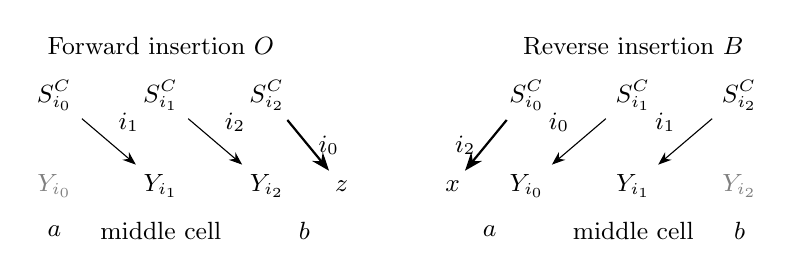
\begin{tikzpicture}[x=1.35cm,y=1.15cm,>=Stealth,
 every node/.style={font=\small}]
 \begin{scope}
  \node at (1,1.55) {Forward insertion $O$};
  \foreach \j in {0,1,2} {
   \node (s\j) at (\j,1) {$S^C_{i_\j}$};
  }
  \node (y1) at (1,0) {$Y_{i_1}$};
  \node (y2) at (2,0) {$Y_{i_2}$};
  \node (z) at (2.7,0) {$z$};
  \node[gray] at (0,0) {$Y_{i_0}$};
  \draw[->] (s0)--node[midway,above right] {$i_1$} (y1);
  \draw[->] (s1)--node[midway,above right] {$i_2$} (y2);
  \draw[->,thick] (s2)--node[midway,right] {$i_0$} (z);
  \node at (0,-.5) {$a$};
  \node at (1,-.5) {middle cell};
  \node at (2.35,-.5) {$b$};
 \end{scope}
 \begin{scope}[xshift=6.0cm]
  \node at (1,1.55) {Reverse insertion $B$};
  \foreach \j in {0,1,2} {
   \node (t\j) at (\j,1) {$S^C_{i_\j}$};
  }
  \node (x) at (-.7,0) {$x$};
  \node (v0) at (0,0) {$Y_{i_0}$};
  \node (v1) at (1,0) {$Y_{i_1}$};
  \node[gray] at (2,0) {$Y_{i_2}$};
  \draw[->,thick] (t0)--node[midway,left] {$i_2$} (x);
  \draw[->] (t1)--node[midway,above left] {$i_0$} (v0);
  \draw[->] (t2)--node[midway,above left] {$i_1$} (v1);
  \node at (-.35,-.5) {$a$};
  \node at (1,-.5) {middle cell};
  \node at (2,-.5) {$b$};
 \end{scope}
\end{tikzpicture}
\caption{Endpoint assignments relative to the same original closed-state starts
$S^C$, for a tuple of three labels in successive
cells. The forward change opens slot $i_0$ at $z\in b$; the reverse
change opens slot $i_2$ at $x\in a$. Gray points remain outer endpoints
but cease to be inner endpoints. Each arrow is labeled by its current
slot and reassigns the original start at its tail to that slot. The two panels
illustrate the single-tuple changes separately; the second-moment comparison
may use different tuples for the forward and reverse changes. Arrows show
only assignments, not sampled
Brownian trajectories or a spatial straightness condition.}
\label{fig:endpoints}
\end{figure}


Identify a tuple with its slot set when taking intersections and
differences, and partition the selected slots as
\[
 \mathsf h=I\cap I',\quad
 \mathsf d=\mathsf h\cup\operatorname{pred}_I(\mathsf h),\quad
 \mathsf j=I\setminus\mathsf d,\quad
 \mathsf l=I'\setminus\mathsf h,\quad
 \mathsf L=(I\cup I')^c .
\]
Thus $\mathsf h$ contains the shared labels, while $\mathsf d$ also
contains their predecessors on $I$. In particular
\(|\mathsf d|\le2|\mathsf h|\) and $e\in\mathsf d$, because the
first label is shared. The two unshared portions that can cancel are
$\mathsf j$ and $\mathsf l$; $\mathsf L$ contains the untouched slots.
Let $J$ count cells of $P$ within distance $R_*$ of $P'$ and conversely,
adding both counts. Call these occurrences near and all others far.

All \(\mathsf L\) paths agree throughout. On \(\mathsf j\), \(C=O\) for endpoints and paths since the slots are off \(I'\), while \(B\) has the endpoints of \(\widehat C\): the \(I\)-successor is not shared, hence also off \(I'\), and \(S_i^B=S_{\operatorname{succ}_I(i)}^C=S_{\operatorname{succ}_I(i)}^O=S_i^{\widehat C}\) there. On \(\mathsf l\), \(B\) has the endpoints of \(C\), and \(\widehat C=O\). The separate path integrations off \(\mathsf L\) and our identification for the comparison are thus:
\[
\begin{array}{c|l|l}
 \text{set} & \text{path variables in (27)} & \text{use in }B\\ \hline
 \mathsf j & C_{\mathsf j}=O_{\mathsf j},\ \widehat C_{\mathsf j}
            & B_{\mathsf j}=\widehat C_{\mathsf j}\ \text{initially}\\
 \mathsf l & C_{\mathsf l},\ O_{\mathsf l}=\widehat C_{\mathsf l}
            & B_{\mathsf l}=C_{\mathsf l}\\
 \mathsf d & C_{\mathsf d},\ \widehat C_{\mathsf d},\ O_{\mathsf h}
            & B_{\mathsf d}\ \text{fresh}.
\end{array}
\]
We will also reintegrate some of \(\mathsf j\) below; \(O\) on \(\mathsf d\setminus\mathsf h\) equals \(C\) there.

We work first on the domain of the original nonzero weights and cuts in (27). All paths there on \(I\cup I'\) in \(C,O,\widehat C\) satisfy \(\mathrm{cut}_R\), by the two cuts in (27) and the two eligibilities. Displacements even for all endpoints needed in conditional integrations are at most \((D+10)s\): in \(O\) use the forward displacement rule from \(C\) on \(I'\) and from \(\widehat C\) on \(I\) (indeed \(S^O=p_I S^{\widehat C}\)). This also covers the non-selected slots on the union in \(C,\widehat C\), which individually have the same endpoints as in \(O\). For \(B\) on \(\mathsf d\), if the successor is shared use its start from an eligible slot of \(C\), close to the successor cell (for \(e\) use that \(x\) is in the first cell); otherwise the start agrees with \(\widehat C\).

For the beginning and end anchors of the integrated rows where (16) is needed the scores against \(\mathsf L\) are \(\le C_0\). In \(O\) the starts on \(I'\) come from eligible starts of \(C\), on \(I\) from eligible starts of \(\widehat C\); the respective end anchors are covered by eligibility or the dummy \(z\) test. Similarly \(B_{\mathsf j},B_{\mathsf l}\) use eligible endpoints from \(\widehat C,C\); on \(\mathsf d\) use the successor rule just given and end eligibility of \(\widehat C\) or the dummy \(x\) test. Paths in \(\mathsf L\) are the same in the scores. Also any pair between \(\mathsf j,\mathsf l\) in \(O\), and in \(B\), has starts separated by more than \(r\) and likewise ends: by the indicated eligible sources the starts used on both sets are isolated in the common start multiset, of which each of \(O,B\) assigns distinct elements (indices) to distinct slots. These ordinary end slots are isolated among \(Y\) by eligibility in \(\widehat C,C\) respectively (no separation from the exceptional inner end is needed).

All confined bridge measures use nearest lifts. Write \(\pi_i^X\) for the probability bridge on that lift before imposing the cut, and factor out the kernels \(k\) of those individual lifts (not the periodic sums), with product denoted \(K_X(G)\) on a set \(G\). Factor the kernels from the cut normalizations as well (write \(\overline{\mathcal Z}\) for the remaining normalization). The proposed-path kernels cancel, and relative to using baseline kernels the ratio left in (27) off \(\mathsf L\) is
\[
 \frac{K_C(I\cup I') K_{\widehat C}(I)}{K_B(I\cup I') K_O(I)}
      =\frac{K_C(\mathsf d)K_{\widehat C}(\mathsf d)}
             {K_B(\mathsf d)K_O(\mathsf d)}\le e^{C|\mathsf h|}.      \tag{28}\label{eq:28}
\]

\subsection{Conditional laws and the two denominator bounds}

For \(G=\mathsf j\) or \(\mathsf l\) write \(\Phi_G^X\) for the exponential of minus the interactions internal to \(G\) and with \(\mathsf L\) only, and \(Z[G,X]\) for its integral with the probability bridges and cuts \(R\), fixing \(\mathsf L\). Use empty-product conventions.

\paragraph{A one-path marginal bound.}
In these normalized group distributions an individual path marginal is bounded by \(C_4\pi_i^X\). The bound also holds if some other paths of the group are frozen on the cut, normalizing conditionally with their interactions. Indeed, conditional on all other paths, the individual normalization for its incident weight is at least \(p_*\) times the exponential of minus the expected interactions under its free bridge conditioned on the cut, by Jensen. Against \(\mathsf L\) use (16) divided by \(p_*\); other confined paths of the group can interact only from nearby end cells (distance at most \(2R+5\)), a bounded number of slots depending on \(R\) by simplicity, and the one-fixed-trajectory expectation bound applies (again divide by \(p_*\)). Thus this incident normalization is at least \(p_* e^{-C/p_*}\). Positivity \(v\ge0\) now gives a uniform conditional density upper bound \(C_4\) relative to \(\pi_i^X\), possibly large but independent of density after fixing the cut and score constants; average the bound for marginals. We use this observation for \(\mathsf j\) with the endpoints of \(C\) (equal to those of \(O\)) or \(B\), and \(\mathsf l\) with those of \(O\).

The needed lower normalizations are
\[
 \begin{split}
     \overline{\mathcal Z}_{I'}(O)&\ge
              Z[\mathsf l,O]\exp[-C|\mathsf h|-o_\rho(1)J],\\
     \overline{\mathcal Z}_{I}(O)&\ge
              Z[\mathsf j,C]\exp[-C|\mathsf h|-o_\rho(1)J].
 \end{split}                                                          \tag{29}\label{eq:29}
\]
Here the small coefficients tend to zero after all cut and eligibility
constants have been fixed. For the first, sample \(\mathsf l\) with its normalized group law, and \(\mathsf h\) independently with product free bridges conditioned on the cuts. Writing \(\mathcal V_{G,G'}\) for the summed interactions between disjoint groups (internal pairs once for \(\mathcal V_{G,G}\)), the ratio to \(Z[\mathsf l,O]\) is the product of free cut probabilities on \(\mathsf h\) times
\[
 \mathbb E\exp[-\mathcal V_{\mathsf l,\mathsf j}
               -\mathcal V_{\mathsf l,\mathsf d\setminus\mathsf h}
               -\mathcal V_{\mathsf h,\mathsf L\cup\mathsf j\cup(\mathsf d\setminus\mathsf h)\cup\mathsf l}
               -\mathcal V_{\mathsf h,\mathsf h}]
\]
with the complement frozen in \(O\). The interaction of \(\mathsf l\) with the frozen \(\mathsf j\) costs at most \(C/\sqrt r\) in expectation per nearby pair: it is zero in the boundary intervals by endpoint separation and both restraints (distance at least \(r-2r/10>R_v\)), and use marginal domination after those intervals. There are at most \(C(R)J\) possible pairs, since end cells must be within \(2R+5\) and are distinct within each set. Interaction with frozen \(\mathsf d\setminus\mathsf h\) costs at most \(C|\mathsf d|\), without needing the small bound. The independently sampled paths cost at most \(C|\mathsf h|\) with \(\mathsf L\) by (16) and with the other integrated or frozen paths by the fixed-trajectory bound and confinement (only a bounded number of slots in a fixed-radius end-cell neighborhood in these latter groups, allowing the special end). Jensen gives the first bound. 

For the second denominator, sample $\mathsf j$ with its group law
(the endpoints of $C$, which agree with those of $O$ on this set),
and sample $\mathsf d$ with independent free cut bridges. The frozen
selected complement is now $\mathsf l$. The missing interactions are
\[
 \mathcal V_{\mathsf j,\mathsf l},\qquad
 \mathcal V_{\mathsf d,\mathsf L\cup\mathsf j\cup\mathsf l},\qquad
 \mathcal V_{\mathsf d,\mathsf d}.
\]
The first sum costs $C r^{-1/2}J$, using the same endpoint separation
in $O$ and the marginal bound for $\mathsf j$. The other sums and the
free cut probabilities cost $C|\mathsf d|\le2C|\mathsf h|$. Jensen's
inequality gives the second line of \eqref{eq:29}.

\paragraph{The remaining normalized factors.}
Using \eqref{eq:28} and \eqref{eq:29}, drop interaction costs from the numerator weights by positivity except for: internal \(\mathsf L\); \(\Phi_{\mathsf j}^C,\Phi_{\mathsf l}^C\) from the closed weight; \(\Phi_{\mathsf l}^O\) from the proposal; \(\Phi_{\mathsf j}^{\widehat C}\) from the hypothetical old weight. 

To spell out the remaining integrations, let \(\pi_G^X\) denote probability-bridge products, \(c_G^X=\mathbf 1_{\mathrm{cut}_R(X_G)}\), and \(d\nu_G^X=c_G^X\Phi_G^X d\pi_G^X/Z[G,X]\) for the normalized groups. Besides the exponential comparison factors, the choice weights/constraints, \(K_B(I\cup I')\) and the original internal measure on \(\mathsf L\), the upper integrand on the nonzero domain now uses
\[
 (c_{\mathsf l}^C\Phi_{\mathsf l}^C\,d\pi_{\mathsf l}^C)
 (c_{\mathsf j}^{\widehat C}\Phi_{\mathsf j}^{\widehat C}\,d\pi_{\mathsf j}^{\widehat C})
 \ d\nu_{\mathsf j}^C\,d\nu_{\mathsf l}^O\,
 d\pi_{\mathsf d}^C\,d\pi_{\mathsf d}^{\widehat C}\,d\pi_{\mathsf h}^O .
\]


In particular the extras \(C_{\mathsf j},O_{\mathsf l}\) occur as normalized factors (fixing just endpoints and \(\mathsf L\) in their laws); all cuts inserted in these measures hold on the original domain. We still account for constraints and far choice weights below. For a near occurrence in cell \(Q\) bound the value of the choice factor on the nonzero domain by \([(1-\varepsilon)n_Q]^{-1}\) for count \(n_Q\) of that outer cell. We can and do carry the indicator of the original constraints (including both nonzero choices) even when bounding such values; in particular the counts along both paths are in the stated occupancy interval there.

\subsection{Restoring the baseline interaction weight}

We describe the weight restoration in \(B\). Put in \(\mathsf j_n\subseteq\mathsf j\) those with end cell within \(2R+5\) of some \(\mathsf l\) cell; other \(\mathsf j\) cannot interact with \(\mathsf l\) on the cuts. 

\paragraph{Fixed data and feasible fibers.}
Throughout this step, all endpoints, tuples, cell paths and skeletons
are fixed. The path integrations divide as follows:
\[
\begin{array}{c|l}
 \text{role}&\text{path variables}\\ \hline
 \text{fixed in both integrals}
   &\mathsf L,\quad B_{\mathsf l}=C_{\mathsf l},\quad
             B_{\mathsf j\setminus\mathsf j_n}
                       =\widehat C_{\mathsf j\setminus\mathsf j_n}\\
 \text{integrated in the original term}
   &\widehat C_{\mathsf j_n},\quad C_{\mathsf j},\quad O_{\mathsf l},
      \quad C_{\mathsf d},\quad\widehat C_{\mathsf d},\quad O_{\mathsf h}\\
 \text{integrated in the baseline term}&B_{\mathsf j_n},\quad B_{\mathsf d}.
\end{array}
\]
Call the fixed data \emph{feasible} if some choice of the remaining
original paths satisfies both nonzero selection weights, their specified
adaptations, and the cuts. Call such a choice a \emph{witness}. We only
need an upper comparison on feasible data: otherwise the original inner
integral vanishes. The probability laws of the extra original paths
depend only on the fixed endpoints and $\mathsf L$, not on
$\widehat C_{\mathsf j_n}$.

\paragraph{Restoring the missing interactions.}
First consider interaction weights alone. The bound needed for replacing
the $\widehat C_{\mathsf j_n}$ integral by a baseline integral is
\begin{equation}
 \Phi_{\mathsf l}^B
      \int c_{\mathsf j_n}^B\Phi_{\mathsf j}^B\,d\pi_{\mathsf j_n}^B
 \ \le\ e^{C|\mathsf h|+o_\rho(1)J}
      \int c_{\mathsf j_n}^B c_{\mathsf d}^B
       \exp\!\Big[-\sum_{\{i,i'\}\not\subseteq\mathsf L}
                          \mathcal V_{ii'}(B)\Big]\,
                       d\pi_{\mathsf j_n}^B d\pi_{\mathsf d}^B ,
\tag{29a}\label{eq:restoring-weights}
\end{equation}
where the sum is over unordered pairs of distinct slots indicated. 

Indeed, normalize
$c_{\mathsf j_n}^B\Phi_{\mathsf j}^B\,d\pi_{\mathsf j_n}^B$ with
$B_{\mathsf j\setminus\mathsf j_n}$ frozen, and independently sample
$\mathsf d$ by free bridges conditioned on their cuts. The earlier
one-path marginal bound applies also to this partially frozen group:
the score against $\mathsf L$ is still bounded, and only boundedly many
frozen or integrated $\mathsf j$ paths can be nearby. The ratio of the
full cut integral on the right to the product on the left is the free
cut probability product on $\mathsf d$, multiplied by the expectation
of the exponential of minus the missing interactions.

The $\mathsf j_n$--$\mathsf l$ interactions cost $o_\rho(1)J$ by
marginal domination, endpoint separation and the boundary restraints.
The frozen remainder of $\mathsf j$ cannot interact with $\mathsf l$
on the cuts. Interactions incident to $\mathsf d$ cost
$C|\mathsf d|$ by the free cut bounds, including \eqref{eq:16}.
Jensen and the cut probabilities prove \eqref{eq:restoring-weights}.
Its endpoint and frozen-path hypotheses follow from original feasibility,
independently of the reintegrated paths.

This inequality concerns interaction weights alone. To apply it to the
original integral, we must still account for the far selection factors
and the path-adaptation constraints. The next step proves that their
needed properties hold for every baseline cut replacement.

\subsection{Tracking the constraints in this comparison}

The original choices depend on which cells are usable and which slots
are eligible. We now compare those tests between any original witness
and every replacement of $B_{\mathsf j_n},B_{\mathsf d}$ on the cuts,
with the other data fixed as above. This universal comparison will
justify using \eqref{eq:restoring-weights} inside the constrained integral.

In $B$, use the outer tuple $Y$, including $Y_e$, for cell counts
and end isolation, and declare the exceptional slot $e$ ineligible.
Other eligibility tests use the starts and paths as before; the
exceptional path is included in all score sums. Let $S_0(B)$ be the
resulting unusable cells. Define $S_1(B)$ by the stricter score threshold
$C_0-\Delta_A$ and the stronger required eligible fraction
$1-\varepsilon/2$, with the same occupancy interval. Thus
$S_0(B)\subseteq S_1(B)$. Write $S(C),S(\widehat C)$ for the
unusable cells in the two witness states. The table compares the tests;
its last column gives the ineligible fraction causing failure when the
count lies in the allowed interval.
\[
\begin{array}{c|c|c|c}
 \text{bad-cell set}&\text{allowed count}&\text{score cutoff}
                                      &\text{failure fraction}\\ \hline
 S(C),S(\widehat C),S_0(B)&[b_-m,b_+m]&C_0&>\varepsilon\\
 S_1(B)&[b_-m,b_+m]&C_0-\Delta_A&>\varepsilon/2\\
 \text{defective cells}
    &[2b_-m,b_+m/2]&C_0-\Delta_A&\ge\varepsilon/4.
\end{array}
\]
Counts outside the displayed interval also cause failure. The symmetric
defective test uses actual inner endpoints, whereas $S_0(B),S_1(B)$
use the outer-end convention just specified. The witness states $C$
and $\widehat C$ are closed, so their inner ends are $Y$.

\begin{lemma}[Stability under every cut replacement]\label{lem:replacement-stability}
Fix feasible endpoint and path data as in the preceding subsection.
For every replacement of $B_{\mathsf j_n},B_{\mathsf d}$ on the cuts
and every original witness $C,\widehat C$, one has
\[
 \begin{gathered}
        S(C),S(\widehat C)\ \subseteq S_1(B),\\
        S(C)=S_0(B)\ \text{pointwise outside distance }R_*\text{ of }P,\\
        S(\widehat C)=S_0(B)\ \text{pointwise outside distance }R_*\text{ of }P'.
\end{gathered}                                                       \tag{30}\label{eq:30}
\]
In the far cells specified by the last two lines, all individual
eligibility indicators and eligible counts agree as well.
\end{lemma}
\begin{proof}
The state $C$ differs from $B$ only on $I$, and $\widehat C$ differs
from $B$ only on $\mathsf l,\mathsf d,\mathsf j_n$. All changed paths
in either comparison are confined. Their slots lie on at most two simple
cell paths, with the special inner end of $B$ in $a$.

At an unchanged slot's anchor, the change in either score is at most
$\Delta_A$. Indeed only changed paths with actual inner ends within
$(R+R_A)s$ of the anchor can contribute. In either state their number
is at most $2(2R+2R_A+4)^3+1$, by outer-cell counting and the one moved
exceptional end; also $\int_0^{\delta/2}w\le3$. Start isolation is
unchanged because the unordered start tuple is unchanged, and ordinary
outer-end isolation is unchanged as well. Consequently the eligible
count in either witness is at least the stricter eligible count of $B$
minus two per outer cell, allowing for the changed slots. If a cell
passes the $S_1(B)$ test, then its witness eligible count is at least
$(1-\varepsilon/2)n_Q-2\ge(1-\varepsilon)n_Q$ for sufficiently large
$m$. The occupancy counts are identical. This proves the inclusion
in \eqref{eq:30} by contraposition.

For exact equality, changed paths comparing with \(C\) lie near \(P\). Comparing with \(\widehat C\), their end cells lie within \(2R+5\) of \(P'\): note \(\mathsf d\) uses shared slots or their predecessors, including the last cell \(b\), and the special end is in \(a\). In a cell beyond the respective distance \(R_*\) there are no changed slots; an unchanged macro-conforming path has both anchors close enough to its cell that scores are exactly unchanged by the indicator cutoff in (15), and a macro failure stays ineligible anyway. The choice of \(R_*\) more than covers these distances. This proves equality of all actual eligibility flags and counts in the respective far cells.
\end{proof}

\paragraph{Lists containing every feasible pair.}
Define an explicit path predicate given \(B,\gamma,\gamma'\). Partition \(S_1(B)\) into components with adjacency distance up to \(K_b=2R_*+10\). Call components bridges if within \(R_*+2\) of both skeletons (set distances), and put \(b_{\rm tot}\) equal to the sum of their sizes. For the list of possible \(P\), take arbitrary subsets of cells in the bridge components as bad; from every nonbridge component intersecting \(\gamma\) take its intersection with \(S_0(B)\) as bad, ignoring the others. Run the deterministic cell-set adaptation for these sets, listing paths when it accepts geometrically. Similarly list \(P'\) using \(\gamma'\). Let \(G\) be the predicate that both given paths are on the respective lists.

The lists depend only on $B,\gamma,\gamma'$; $G$ tests membership of
the given cell-path pair and has no further dependence on its labels.

\begin{lemma}[Path lists and their encounter bound]\label{lem:path-lists}
For every original witness and every baseline cut replacement in
Lemma~\ref{lem:replacement-stability}, the witness paths $P,P'$ satisfy
$G$. For arbitrary $B$, the lists contain at most $4^{b_{\rm tot}}$
path pairs. Every listed pair satisfies
\[
                       J\le J_0+C(R_*)b_{\rm tot}.
                       \tag{31}\label{eq:32}
\]
Here $J_0$ counts encounters of the original skeletons, as in
Lemma~\ref{lem:skeleton}.
\end{lemma}
\begin{proof}
First fix a witness and any cut replacement. A nonbridge component of
$S_1(B)$ intersecting $\gamma$ stays outside distance $R_*$ of $P'$.
If it approached a skeleton vertex of $P'$, it would be a bridge. If it
approached a detour vertex, it would join, in the $K_b$ adjacency, the
potential component containing that detoured obstacle, which is hit by
$\gamma'$. It would again be a bridge. Therefore \eqref{eq:30} identifies
the actual bad subset of $\widehat C$ on this whole nonbridge component
as its intersection with $S_0(B)$.

On bridge components, choose the guessed subsets to be the actual bad
cells of $\widehat C$. Every actual nearest-neighbor bad component lies
in a single $K_b$-component of $S_1(B)$, and every such component hit by
$\gamma$ is retained. The reconstructed set therefore removes only whole
actual bad components not hit by $\gamma$. Lemma~\ref{lem:detour}
preserves acceptance and the adapted path under precisely these
deletions. Hence $P$ is listed. The same argument with $C,\gamma'$
gives $P'$. This reasoning holds for every replacement.

There are at most $2^{b_{\rm tot}}$ guesses for each path, giving
$4^{b_{\rm tot}}$ pairs. To bound their encounters, first count near
occurrences that lie on their own skeleton and have an opposite-skeleton
vertex within distance $R_*$. Since the adapted paths are simple, these
occurrences inject into the corresponding counts of $J_0$.

Every remaining near occurrence is a detour vertex or is close to an
opposite detour vertex. Any detour participating in such an encounter
belongs to a bridge component: it is adjacent to its obstacle, which
is hit by its skeleton, and either lies close to the other skeleton or
joins the component of an opposite detoured obstacle in the $K_b$
adjacency. Across both paths, these detours use at most $12b_{\rm tot}$
vertices by Lemma~\ref{lem:detour}. Their fixed-radius neighborhoods
contain at most $C(R_*)b_{\rm tot}$ cells. Simplicity bounds the number
of path occurrences in those cells by twice this number. This proves
\eqref{eq:32} with coefficient one on $J_0$. The argument also applies
to guessed subsets: their nearest-neighbor obstacles remain within
components of $S_1(B)$.
\end{proof}

\paragraph{The common far-choice product.}
For a slot, its choice factor in $B$ is its eligible indicator divided
by the eligible count in its outer cell, using the $S_0(B)$ criteria
and assigning zero when the count is zero. Let $H_F(B)$ be the product
of these factors for the selected far occurrences of both paths.
Unlike the path lists, this product depends on the selected labels.
Its indicators and denominators are nevertheless all evaluated on the
same fixed baseline configuration.

Lemma~\ref{lem:replacement-stability} identifies these factors exactly
with the original far factors: $P$ uses $\widehat C$ and $P'$ uses $C$.
At feasible fixed data their product therefore has a common value
$H_*$ for all original witnesses and all cut replacements. Indeed,
the equality holds between \emph{any} witness and \emph{every}
replacement, and the replacement cuts are nonempty. This is the
selection property needed to apply \eqref{eq:restoring-weights}.



Explicitly, at those fixed variables let \(\mathcal D\) impose the original remaining constraints, \(H_{\rm old}\) be the far product there, and use the product probability measure
\[
d\mathcal P=d\nu_{\mathsf j}^C\, d\nu_{\mathsf l}^O\,
 d\pi_{\mathsf d}^C\,d\pi_{\mathsf d}^{\widehat C}\,d\pi_{\mathsf h}^O
\]
on the extras (its laws do not depend on the integrated \(\widehat C_{\mathsf j_n}\)). Having bounded the near factors, the needed inequalities on feasibility, omitting the cut indicators equal to one on the fixed paths in \(\mathsf j,\mathsf l\), are
\[
\begin{split}
 &\Phi_{\mathsf l}^B
 \int c_{\mathsf j_n}^{\widehat C}\Phi_{\mathsf j}^{\widehat C}
       \mathbf 1_{\mathcal D} H_{\rm old}\,d\pi_{\mathsf j_n}^{\widehat C}\,d\mathcal P\\
 &\quad\le H_*\,\Phi_{\mathsf l}^B
      \int c_{\mathsf j_n}^B\Phi_{\mathsf j}^B\,d\pi_{\mathsf j_n}^B\\
 &\quad\le e^{C|\mathsf h|+o_\rho(1)J}
      \int c_{\mathsf j_n}^B c_{\mathsf d}^B
       \exp\!\Big[-\sum_{\{i,i'\}\not\subseteq\mathsf L}
                          \mathcal V_{ii'}(B)\Big]\mathbf 1_G H_F(B)\,
                       d\pi_{\mathsf j_n}^B d\pi_{\mathsf d}^B .
\end{split}
\]
The first inequality removes the original constraints only after
factoring out their common far product. The second uses
\eqref{eq:restoring-weights} and Lemma~\ref{lem:path-lists}:
$\mathbf1_GH_F(B)=H_*$ everywhere on the cut replacements. At
infeasible data the original inner integral is zero, so its comparison
with the nonnegative baseline integral is automatic. Thus the argument
compares inner integrals at fixed data, without choosing replacements
according to the number of witnesses they admit.

For precision, denote the original conditional path integral by
\[
\begin{split}
 \mathcal I_{I,I'}={}&\int W(C)h_{\gamma'}(C,I')
 \frac{\mathbf1_{\mathrm{cut}_R(O_{I'})}W_{I'}^O}
      {\mathcal Z_{I'}(O)}\\
 &\hspace{5mm}\cdot
 \frac{\mathbf1_{\mathrm{cut}_R(O_I)}}{\mathcal Z_I(O)}
                    W_I^{\widehat C}h_\gamma(\widehat C,I).
\end{split}
\]
The integrations are over the original closed paths, proposed paths on
$I'$, and hypothetical old paths on $I$, with the endpoints, tuples, and
skeletons fixed. Let $\mathbf1_{\mathrm{occ}}$ require that the outer
counts lie in $[b_-m,b_+m]$ in every cell of both paths.

\begin{lemma}[Integrated cross comparison]\label{lem:cross}
Fix two simple star cell paths from $a$ to $b$, their label tuples
matching the outer $Y$-cells and having a common first label,
two skeletons, and endpoint data $Y,S^C,x,z$ as in \eqref{eq:27}.
With $B$, the near occurrences, $G$, and $H_F(B)$ defined above, one has
\[
\begin{split}
 \mathcal I_{I,I'}\le{}&
 e^{C|\mathsf h|+\sigma_\rho J}\mathbf1_{\mathrm{occ}}
 \prod_{\substack{\text{near occurrences}\\\text{in cell }Q}}
                              [(1-\varepsilon)n_Q(Y)]^{-1}\\
 &\hspace{8mm}\cdot\int W(S^B,E^B;d\omega)\,\mathbf1_G H_F(B).
\end{split}\tag{32}\label{eq:31}
\]
Here $C<\infty$ is fixed and $\sigma_\rho\ge0$ tends to zero as
$\rho\downarrow0$ after the cutoffs are fixed, uniformly in all permitted
volumes and temperatures. A cell on both paths is counted twice in the
product. The right side is zero when the occupancy condition fails.
\end{lemma}
\begin{proof}
The preceding inner-integral comparison proves the displayed bound on
every feasible fiber. On an infeasible fiber the original contribution
is zero. We explain the remaining bookkeeping to specify precisely how
the full integral is recovered.
Keep $\mathsf L,B_{\mathsf l},B_{\mathsf j\setminus\mathsf j_n}$ fixed
and integrate the extensions in $\mathsf j_n,\mathsf d$ as in the
displayed ledger. Whenever the original domain is nonempty, all the
nearest-kernel factorizations apply. Restore the baseline kernels from
\eqref{eq:28}, then integrate the fixed paths. Finally drop the remaining
cut and nearest-lift restrictions from the baseline integral by
positivity, obtaining \eqref{eq:31}. Its predicates are measurable
functions of the baseline paths, specified by finite cell algorithms.
This use of the conditional comparison is valid pointwise at the fixed
data: a positive original inner integral has a witness, and otherwise
the required upper bound is automatic.

\end{proof}

The conditional comparison is now established. To average its path-list
cost, we need the defect bound under the reverse insertion. Under
$\mu_{ab}$, with $e$ the opened slot in each term, every specified
cell set $\mathcal U$ satisfies
\[
                  \mu_{ab}(\mathcal U\subseteq S_1(B))
                              \le C M^{-2} q^{|\mathcal U|},
                  \qquad q=q_{\rm cl}^{1/4},                          \tag{33}\label{eq:33}
\]
including the empty set bound. To compare to the symmetric defective test replace the exceptional outer endpoint by its actual inner end for counting and isolation. Counts change by at most one; only a bounded number of other end-isolation flags can change: those isolated before but not after are mutually separated by more than \(r\) and within \(r\) of the new point, and analogously in reverse (use packing). Their other tests are unchanged. Allow also the exceptional slot itself. For a potential bad cell with count \(n_Q(Y)\) in the occupancy interval, the ineligible count in the actual stricter-score test is thus at least \((\varepsilon/2)n_Q(Y)-C\), giving at least fraction \(\varepsilon/4\) for large \(m\); counts outside the interval imply the widened count defect after any change by one. This works pointwise in all the specified cells. Now apply \eqref{eq:22} and \eqref{eq:23}.

\subsection{Summing the comparison}

The conditional comparison is now complete, including its selection
predicates. We sum first over labels at fixed baseline paths, then over
the finite lists of possible cell paths. The remaining environment
average will be controlled by the insertion defect bound and the two
skeleton moments.

\paragraph{Summing label choices.}
Sum \eqref{eq:31} over candidate cell-path pairs and their tuples; this
candidate range depends on $a,b,Y$, but not on the starts. For each
tuple pair change variables from $S^C$ to $S^B$. The outer kernel is
invariant. Group terms by the last label $e$ of $I$, whose outer end
lies in $b$. At fixed $e$ and baseline configuration, the baseline
measure, $S_0,S_1$, and the path lists are independent of every other
label choice.

Fix a listed pair satisfying the occupancy bound. A far cell occurs on
only one path, and summing its choice factor from $H_F(B)$ costs at
most one. Each near occurrence contributes a factor
$(1-\varepsilon)^{-1}$. After removing these factors, the remaining
cellwise sums are
\[
\begin{array}{c|c|c}
 \text{cell}&\text{label choices}&\text{upper bound}\\ \hline
 \text{ordinary common cell }Q&\text{two independent labels}
       &1+(e^C-1)/n_Q\\
 \text{first cell }a&\text{one shared label}&e^C/n_a\\
 \text{last cell }b&\text{first tuple's label fixed to }e
       &[1+(e^C-1)/n_b]/n_b.
\end{array}
\]
For example, at an ordinary common cell, the $n_Q$ coincident choices
carry $e^C$ and the $n_Q(n_Q-1)$ distinct choices carry one, all divided
by $n_Q^2$. At $a$ the two tuples must share their first label; at $b$
one of the two labels is fixed by the grouping. The endpoint cells are
distinct. Simplicity makes these sums independent across cells, since
labels in different outer cells cannot coincide. Using $n_Q\ge b_-m$
and including $e^{\sigma_\rho J}$ gives the bound
\[
                           \frac{C}{m^2}e^{\kappa_0 J},
                       \qquad \kappa_0=2\varepsilon+o_\rho(1).
\]
Lemma~\ref{lem:path-lists} now sums the cell-path pairs, giving
$C m^{-2}\exp(\kappa_0J_0+C'b_{\rm tot})$ with fixed $C'$.

\paragraph{Recovering the reverse insertion.}
There is no remaining dependence on the dummy-for-\(B\) point \(z\) within \(b\); its base integral there gives \(1/M\). Together with the prefactor of (27) we have \(m/(m^2 M)=1/N\); summing \(e\) with \(Y_e\) in \(b\) and integrating the baseline with \(x\) in \(a\) using \(dx/V\) now gives exactly $\mu_{ab}$, with outer endpoint in $b$ and new
inner endpoint in $a$, as defined in Section~\ref{sec:defects}. Thus
\[
                 \int f^2\dd\mu
         \le C\sum_{a,b\ {\rm valid}} \mathbb E_{\gamma,\gamma'}\!
               \left[e^{\kappa_0 J_0}
                   \int e^{C' b_{\rm tot}}\,d\mu_{ab}\right].         \tag{34}\label{eq:34}
\]

\paragraph{The exponential moment of rare components.}
For fixed skeletons, we claim
\[
 \int e^{C'b_{\rm tot}}\,d\mu_{ab}
 \le \frac C{M^2}\exp\!\left[\vartheta(q)S_{K_b}\right],
 \qquad \vartheta(q)\longrightarrow0\quad(q\downarrow0),
\]
where $S_{K_b}$ is the soft-distance sum of Lemma~\ref{lem:skeleton}.
This is the estimate that allows the environment average in
\eqref{eq:34} to use the second skeleton moment.

Expand the product over realized bridge components of $S_1(B)$ with
factors $1+(e^{C'|T|}-1)$. Bound it by the sum over unordered
collections of disjoint connected sets $T$ in the $K_b$ adjacency,
each within $R_*+2$ of both skeletons, requiring their cells to lie in
$S_1(B)$. Apply \eqref{eq:33} to each union. Summing the products and
then dropping disjointness gives
\[
                   C M^{-2}
                     \exp\Big(\sum_T(e^{C'}q)^{|T|}\Big)
\]
(the sum in the exponent is over individual qualifying sets). 

Root their counting near vertex occurrences \(z\in\gamma\); there are a bounded number of root cells per occurrence and at most \(C(K_b)^j\) connected sets of size \(j\) per root by the bounded degree. To reach the other skeleton requires \(d_\infty(z,\gamma')\le 2(R_*+2)+K_b j\). Consequently the exponent sum is at most
\[
                        o_q(1)\sum_{z\in\gamma}
                                     e^{-d_\infty(z,\gamma')/K_b}
\]
by a geometric series: per root sum \((C(K_b)e^{C'}q)^j\) only at sizes with \(d_\infty(z,\gamma')/K_b\le j+2(R_*+2)/K_b\), extracting the displayed distance decay. 

The geometric-series bound proves the claim with a coefficient
$\vartheta(q)\to0$. Take density small enough that $2\kappa_0\le\alpha$
and $2\vartheta(q)\le\xi(K_b)$. Cauchy--Schwarz and
\eqref{eq:24}--\eqref{eq:25} then give, for each valid pair,
\[
 \mathbb E_{\gamma,\gamma'}
 \left[e^{\kappa_0J_0}\int e^{C'b_{\rm tot}}\,d\mu_{ab}\right]
 \le \frac C{M^2}
       \bigl(\mathbb Ee^{2\kappa_0J_0}\bigr)^{1/2}
       \bigl(\mathbb Ee^{2\vartheta(q)S_{K_b}}\bigr)^{1/2}
 \le \frac C{M^2}.
\]
There are at most $M^2$ ordered pairs. Substitution into
\eqref{eq:34} proves Proposition~\ref{prop:second-moment}.

\section{Choice of constants and the limits}\label{sec:conclusion}

We assemble the finite-volume estimate and make its uniformity explicit.
The cutoffs are fixed from the potential before the density is reduced;
the volume threshold is chosen afterward at each fixed density. This
order also permits the zero-temperature limit at fixed volume.

\begin{proof}[Proof of Theorem~\ref{thm:main}]
The change of measure in Section~\ref{sec:opening} has mass at least
$\upsilon/2$. Proposition~\ref{prop:second-moment} gives
$\int f^2\dd\mu\le C_v$,
where $C_v$ is independent of $\rho,L,N,T$ after the fixed cutoff choices.
Since $\mu$ has total mass $q_0$, Cauchy--Schwarz yields
\[
 q_0\ge \frac{\upsilon^2}{4C_v}=:c_*(v)>0.
\]
We specify why all choices can be made without introducing density
or temperature dependence into this constant.

Choose the parameters in this order.
\begin{enumerate}[label=\textup{(\arabic*)}]
\item Fix the localization multipliers in the upper density estimates,
reserving the positive energy fraction used for isolation in
\eqref{eq:13}. Fix the small particle-addition fraction $\eta$, then
$K$ large enough for the lower density estimate, and then the occupancy
constants $b_-,b_+$.
\item Choose the macro cutoff $D$ large, with
$\varepsilon=\alpha(D)/20$ as in Lemma~\ref{lem:skeleton}.
The quantity $\alpha(D)$ decreases only polynomially in $D$, whereas
the macro failure bound in \eqref{eq:17} decreases as a Gaussian tail.
Thus both the marked-color gap condition and the required macro
smallness for \eqref{eq:22} hold.
\item Choose $\zeta>0$ small enough for the isolation tail, and then
$C_0$ large enough for the joint score tails and the two uniform dummy
anchor tests. All these constants are now fixed, depending only on $v$.
\item Decrease $\rho_*(v)$ to satisfy every small-density restriction.
In particular $r=\zeta\rho^{-1/3}$, $m\asymp\rho^{-1/2}$, and
$\lambda_0m=r\sqrt\rho\,m\asymp\rho^{-1/3}$ tend to infinity.
The joint defect parameter tends to zero. Fixed conditional bridge
bounds may be large, but the encounter terms they multiply contain
$r^{-1/2}$ or $m^{-1}$ and hence tend to zero. Therefore
$2\kappa_0\le\alpha$, and twice the coefficient in the soft-distance
component bound is within the threshold of \eqref{eq:25}.
\item At each $\rho<\rho_*(v)$ choose $L_0(\rho,v)$ large enough for
all torus lifts, grids, and geometric rejection bounds. None of these
conditions requires a further temperature restriction within
$0<T\le\rho^2$.
\end{enumerate}
This gives the claimed finite-volume lower bound at positive temperature.

At fixed such $N,L$, the labelled Schr\"odinger semigroup is positivity
improving: the free heat kernel is strictly positive and the bounded
interaction gives a strictly positive Feynman--Kac weight.
Compact resolvent and positivity improvement give a unique positive
normalized ground eigenfunction. Permutation invariance then makes it
symmetric, so it is also the unique bosonic ground state. The normalized
Gibbs state converges in trace norm to its projector as
$\beta\to\infty$. The occupation observable
$N^{-1}\sum_i(|u_0\rangle\langle u_0|)_i$ is bounded by one;
its expectation therefore converges as well. The lower bound, already
uniform over $\beta\ge\rho^{-2}$, survives at $T=0$.

Finally fix $\rho$ and $T$ in the stated ranges. Every sequence with
$L\to\infty$ and $N/L^3\to\rho$ eventually satisfies both the density
band and the volume threshold. The same $c_*(v)$ applies to each late
member, proving the asserted lower limit.
\end{proof}

\bibliographystyle{plainnat}
\bibliography{references}
\end{document}
